\documentclass[12pt]{article}
\usepackage{bigpage}
\usepackage{mathsx,tech,mytheorems}
\usepackage{tikz}
\usetikzlibrary{arrows}
\usepackage{scalalistings}%\unScalaMid

\newtheorem{lemma}{Lemma}
\newtheorem{prop}[lemma]{Proposition}
\newtheorem{corollary}[lemma]{Corollary}
\newtheorem{conjecture}[lemma]{Conjecture}
\newtheorem{definition}[lemma]{Definition}
\newtheorem{example}[lemma]{Example}
\newtheorem{assumption}[lemma]{Assumption}

\newtheorem{improve}{IMPROVE}
\newtheorem{impNote}{Implementation note}
\newtheorem{opt}{Optimisation}

\def\vec#1{\mathsf{#1}}
\def\trans#1{\stackrel{#1}\rightarrow}
\def\sqge{\sqsupseteq}
\def\sqle{\sqsubseteq}
\def\rangeRes{\rhd}
\def\domRes{\lhd}

\def\id{\mathrm{id}}
\def\params{\mathrm{params}}
%\def\srv{\vec{srvs}}
\def\fixed{\mathrm{fixed}}
\def\cpt{\mathrm{cpts}}
\def\cpts{\cpt}
\def\princ{\mathrm{princ}}
\def\S{\mathcal{S}}
\def\V{\mathcal{V}}

\def\mit{\it}

%\def\improve#1{IMPROVE: \emph{#1}}
%\def\impNote#1{\textbf{Implementation note:} #1}

%\def\floatpagefraction{0.85} 
\def\topfraction{0.9}

\everymath{\it}
\sloppy

\title{Reference-Oriented View Abstraction: Working Paper}
\author{Gavin Lowe}

\begin{document}
\maketitle



\section{Setting}

Assume a state machine for each individual process. 

Each process state is a pair $(cs, ps)$ where $cs$~is a control state and $ps$
is a vector of parameters.  The first parameter of a component is always its
own identity.  Other parameters are references to other components.  For the
fixed process, all parameters are references to components.  Write $p.cs$ and
$p.\params$ for the control state and parameters of process state~$p$.  If $p$
is a component state, write $p.\id$ for its identity.
  
%%  We say that $s$ \emph{references} $id'$ if $id'$ is a parameter of~$s$
%% other than its own identity.

Write a system state as $s = (\fixed, \cpt)$ where $\fixed$ is the state of
the fixed process, and $\cpt$ is a set of states of components.  Write $\S$
for the set of all system states.  Write $s.\fixed$ and $s.\cpt$ for the fixed
processes or components, respectively.

If $s$ is a system state and $cpts$ is a set of component states with identities
disjoint from $s.\cpt$, then write $s \uplus cpts$ for $(s.\fixed, s.\cpt \union
cpts)$.  If $cpt$ is a component state, we abuse notation and write $cpt \in
s$ for $cpt \in s.\cpt$.

Assume different components have different identities for now. 

%% If $id$ is an identity, we say that $id$ is in $s$ if there is a
%% component~$cpt \in s$ such that $s.\id = id$.  We say that $s$ references $id$
%% if a component of~$s$ references~$id$. 

Assume that components are partitioned into \emph{active} and \emph{passive}
components.  E.g.~threads and nodes.  Each transition involves precisely one
active component or an active fixed process. 

\improve{check this in implementation.}


\section{View abstraction}

Define views as substates.
\begin{eqnarray*}
(\fixed, \cpt ) \sqle (\fixed', \cpt') & iff & 
  \fixed = \fixed' \land \cpt \subseteq \cpt' .
\end{eqnarray*}

%% Assume $\S$ is downwards-closed under taking substates. 

Fix a set $\V \subseteq \S$ of views.

Given a system state $s$, let
%
\begin{eqnarray*}
\alpha(s) & = &
  \set{ v | v \in \V \land v \sqle s}.
% \set{view(s, cpt) | cpt \in s.\cpt} \union \set{srvView(s)}.
\end{eqnarray*}
%
Lift to sets of states by pointwise application. 

Given a set $V$ of views
\begin{eqnarray*}
\gamma(V) & = &   \set{ s | s \in \S \land \alpha(s) \subseteq V }.
\end{eqnarray*}



\begin{lemma}
If $S, S' \subseteq \S$ and $V, V' \subseteq \V$, then
\begin{enumerate}
\item $S \subseteq S' \implies \alpha(S) \subseteq \alpha(S')$;

\item $V \subseteq V' \implies \gamma(V) \subseteq \gamma(V')$;

\item $\alpha(\gamma(V)) \subseteq V$;

\item $S \subseteq \gamma(\alpha(S))$.
\end{enumerate}
\end{lemma}
%
%% \begin{proof}
%% First two immediate.

%% Suppose $v \in \alpha(\gamma(V))$.  Then $v \in \alpha(s)$ for some $s \in
%% \gamma(V)$.  But then $\alpha(s) \subseteq V$, so $v \in V$.

%% Suppose $s \in S$.  Then $\alpha(s) \subseteq \alpha(S)$ so $s \in
%% \gamma(\alpha(S))$. 
%% \end{proof}

\begin{lemma}
$(\alpha, \gamma)$ forms a Galois connection: if $S \subseteq \S$ and $V
  \subseteq \V$ then $\alpha(S) \subseteq V \iff S \subseteq \gamma(V)$.
\end{lemma}
%
%% \begin{proof}
%% Suppose  $\alpha(S) \subseteq V$.  Then $S \subseteq \gamma(\alpha(S))
%% \subseteq \gamma(V)$.

%% Suppose $S \subseteq \gamma(V)$.  Then $\alpha(S) \subseteq \alpha(\gamma(V))
%% \subseteq V$.
%% \end{proof}


Other things go through as before.  

\begin{definition}
Two views $v$ and~$v'$ are \emph{accordant} if (1)~$v.\fixed = v'.\fixed$, and
(2)~if $v$ and~$v'$ both contain a component with a particular identity~$id$,
then those components are equal.  In this case we write $v \uplus v'$ for
$(v.\fixed, v.\cpts \union v'.\cpts)$.  
\end{definition}

\section{Reference-oriented views}
\label{sec:views}

We now define the set of views we use in our approach.  We say that a process
state $q$ \emph{references} a component state~$c$ if $c.\id \in q.\params$.
Note that $c.\id$ is not a distinguished value.

Consider a system state $s$, and a particular component $p \in s.\cpts$.  We
write $view(s, p)$ for the view of the system state from~$p$, i.e.~the
fixed processes of~$s$, and all the components of~$s$ to which $p$ has a
reference (including itself):
%
%% Let $\cpts' = \set{c \in \cpts | c.id \in cpt.params}$ be all
%% components in $\cpts$ that are referenced by $cpt$ (including $cpt$ itself).
%% We define the corresponding view to be $(\fixed, \cpt')$.  Write this as
%% $view(s, cpt)$.  
%
\begin{eqnarray*}
view(s, p) & = &
  (s.\fixed, \set{c \in s.\cpts \| c.\id \in p.\params}).
\end{eqnarray*}
%
We say that $p$ is the \emph{principal component} of this view, and the
other components are \emph{secondary components}.  Given a view~$v$, we write
$v.\princ$ for its principal component. 

We then define the set~$\V$ of views and the abstraction function~$\alpha$ in
terms of all such views.
%
\begin{eqnarray*}
\alpha(s) & = & \set{ view(s, p) \| p \in s.\cpts } \\
\V & = & \Union_{s \in \S} \alpha(s)
\end{eqnarray*}

In examples, we will write views by listing their fixed components in some
standard order, then listing the components with the principal first, and then
following the order of the references in the principal's parameters.  (Our
implementation uses the same order.)  For instance, in the example of
Figure~\ref{fig:lock-based-queue}, the views will include,
\[
\begin{align}
(\Lock'(t), \Head(n_h), \Last(n_l), \Con_3; 
  Enq_4(t, n_l, n), \Node_y(n_l, null),\Node_x(n, n_l)),
\end{align}
\]
for $t \in ThreadID$, $n_h, n_l, n \in NodeID$, and~$x, y \in D$.  Here the
principal~$t$ has references to~$n_l$ and~$n$, so the two corresponding nodes
are included as secondary components.
Likewise, the following would be a view of the node~$n_1$:
\[
(\Lock'(t), \Head(n_h), \Last(n_l), \Con_3; \Node_x(n_1, n_2), \Node(n_2, n_3)).
\]

The initial views $AInit$ are of the form
\[
\begin{array}{ll}
(\Lock, \Head(null), \Last(null), \Con_0; Thread(t)), &
   \mbox{for $t \in ThreadID$}, \\
(\Lock, \Head(null), \Last(null), \Con_0; \InitNode(n)), & 
   \mbox{for $n \in NodeID$}.
\end{array}
\]
This satisfies the condition $\alpha(Init) \subseteq AInit$ of
Proposition~\ref{prop:reachable}, where $Init$ is the set of initial system
states from Section~\ref{sec:setting}.

For examples based on Figure~\ref{fig:lock-based-queue}, in the interests of
conciseness, we define
\begin{eqnarray*}
fixed(t, n_h, n_l) & = & (\Lock'(t), \Head(n_h), \Last(n_l), \Con_3), \\
fixed(\_, n_h, n_l) & = & (\Lock, \Head(n_h), \Last(n_l), \Con_3).
\end{eqnarray*}
%
These are fixed processes where: the head and last nodes are $n_h$ and~$n_l$;
the lock is held by~$t$ or not held (respectively); and the constructor has
completed.

Note that if one of the principal's parameters is a distinguished value, then
there is no corresponding component in the view.  For example, the following
would be a valid view of node~$n$, whose |next| reference is the distinguished
value~|Null|: 
%% , where the thread's second reference is the distinguished value~$Null$ (in
%% fact, no such state is reachable in the lock-based queue example).
\[
(fixed(t, n_h, n_l);  \Node_x(n, Null)).
\]


%% We let $\V$ be the set of all views of system states:
%% %
%% \begin{eqnarray*}
%% \V & = & 
%%   \set{view(s, cpt) \| s \in \S, cpt \in s.\cpt}. %%  \union 
%%   %% \set{srvView(s) | s \in \S}.
%% \end{eqnarray*}
%% %
%% In the following, we use the word ``view'' for a member of~$\V$, and the word
%% ``substate'' (or just ``state'') for a general substate of an element of~$\S$.

%%%%%%%%%%%%%%%%%%%%%%%%%%%%%%%%%%%%%%%%%%%%%%%%%%%%%%%

% \subsection{Calculating abstract transitions}

{prop:reachable}

The critical thing. in order to apply Proposition~\ref{prop:reachable}, is
that given $V \subseteq \V$, we need to calculate a representation of
%
\begin{eqnarray*}
aPost(V) & = & \alpha(post(\gamma(V)))
\end{eqnarray*}
efficiently.  In fact, we slightly over-estimate $aPost(V)$.  To this end, we
need to deal with the following difficulties.
%
\begin{itemize}
\item Since we are dealing with an infinite number of systems, we need to deal
  with an infinite number of views.  Indeed, even the set of initial views,
  described above, is infinite, since the types of thread and node identities
  are unbounded.  We will deal with this using symmetry reduction.  If two
  views are symmetric to one another, i.e., one can be obtained from the other
  by a uniform remapping of parameters, then the subsequent behaviours of one
  can be deduced from the behaviours of the other: in particular, if one is
  error-free, then so is the other.  Thus it will be enough to consider just
  one of them, or, more generally, just one element of each symmetry
  equivalence class.  We will formalise these ideas in
  Section~\ref{sec:symmetry}.

\item Even if $V$ is finite, the set $\gamma(V)$ can become very large.  We
  want to calculate an upper bound to $aPost(V)$ without calculating all of
  $\gamma(V)$.  We describe how to do this in Section~\ref{sec:transitions}. 
\end{itemize}

%% We are seeking to identify views~$v$ such that
%% \[
%% \gamma(V) \ni s \trans{a} s' \sqge_\V v
%% \]
%% for some $s$, $s'$, $a$.



%%%%%%%%%%%%%%%%%%%%%%%%%%%%%%%%%%%%%%%%%%%%%%%%%%%%%%%

\section{Symmetry reduction}
\label{sec:symmetry}


Idea of symmetry reduction.

\begin{definition}
We define a \emph{renaming} function to be a partial injective function~$\pi$
over non-distinguished parameters, that preserves types (for example, maps
each node identity to a node identity, and each thread identity to a thread
identity).

If $\pi$ is a renaming function defined over the parameters of a component
state~$s$, then we write $\pi(s)$ for the effect of replacing each
parameter~$x$ of~$s$ by~$\pi(x)$.  We extend this to sets of states, views,
etc., by pointwise application.  For example, given
%
\begin{eqnarray*}
v & = & 
  \begin{align}
  (\Lock'(T_1), \Head(N_0), \Last(N_1), \Con_3; \\
  \qquad  Enq_4(T_1, N_1, N_3), \Node_y(N_1, null),\Node_x(N_3, N_1))
  \end{align} \\
\pi & = & 
  \set{ T_1 \mapsto T_0, N_0 \mapsto N_1, N_1 \mapsto N_2, N_3 \mapsto N_0 },
\end{eqnarray*}
%
we have 
\begin{eqnarray*}
\pi(v) & = & 
  \begin{align}
  (\Lock'(T_0), \Head(N_1), \Last(N_2), \Con_3; \\
  \qquad Enq_4(T_0, N_2, N_0), \Node_y(N_2, null),\Node_x(N_0, N_2)) .
  \end{align}
\end{eqnarray*}
\end{definition}

%%%%%

\begin{definition}
Given two views~$v$ and $v'$, we say that~$v$ and~$v'$ are \emph{equivalent},
written $v \equiv v'$, if there is a renaming~$\pi$ such that $\pi(v) = v'$.
Note that this is an equivalence relation.
\end{definition}

%%%%%

\framebox{Explain} why it's enough to store views, up to equivalence.  As in
previous paper. 

We represent each equivalence class of views by a single representative.  More
precisely, we define a normal form of views, and take the representatives to
be the views in normal form: there will be one per equivalence class.  We
describe the normal form below. 

For each type of identities, we assume a linear order over the type.  In
examples below, for node identities we will assume an order $N_0 < N_1 <
N_2 < \ldots$; and similarly for thread identities.  (In the implementation,
identities are represented by non-negative integers: we use the integer
order.)

The following definition captures our normal form.
%
\begin{definition}
Within views, extended views, etc., we use a standard order for the fixed
processes (in the implementation, this order is defined in the input script).
We order components in the order we have been using in examples: principal
first, followed by secondary components in the order corresponding to the
references from the principal (without repetitions).  For extended views, any
additional component is added at the end.  

Given this ordering or processes, we say that a view or extended view is in
\emph{normal form}, if for each type, the first occurrences of each parameter,
when read from left to right, form an initial segment of that type (according
to the linear order described above).

A transition $pre \trans{} post$ is in normal form if $pre$ is in normal form,
the components of~$post$ are in the same order as for~$pre$ (so $post$ itself
might not be in normal form), and the first occurrences of each parameter
within the concatenation of $pre$ ad $post$ form an initial segment of that
type.
\end{definition}

For example, the following view is in normal form; we have underlined the
first occurrence of each parameter.
\[
\begin{align}
(\Lock'(\underline{T_0}), \Head(\underline{N_0}), 
    \Last(\underline{N_1}), \Con_3; 
  Enq_4(T_0, N_1, \underline{N_2}), \Node_y(N_1, null),\Node_x(N_2, N_1)) .
\end{align}
\]

\framebox{Example} of transition in normal form. 

A view can be reduced to normal form by a simple left-to-right traversal,
keeping track of the renaming built so far, and extending it to map the first
occurrence of each parameter to the first unused parameter of that type.

%% \begin{lemma}
%% \label{lem:normal-form-fixed}
%% If $s$ and~$s'$ are both in normal form, and $\pi(s)$ and~$\pi'(s')$ are
%% substates of the same system state, then $s.\fixed = s'.\fixed$.
%% \end{lemma}

\section{Calculating induced transitions with symmetry reduction}
\label{sec:induced-symmetry}

In this section, we consider consider how to calculate the transition induced
by a transition $pre \trans{e} post$ on a view~$v$, given that both are in
normal form and represent all members of their equivalence classes.  
%
Following Definition~\ref{def:induced-transition}, in principle, we need to
find all ways of renaming parameters of~$v$ and~$pre$ to produce views that
are accordant.  However, if two different renamings would produce equivalent
post-views, it is enough to consider just one of them.  It is therefore enough
to keep the parameters of $pre$ fixed, and to rename the parameters of~$v$.
Each renaming can be defined by an renaming~$\pi$ over the parameters of~$v$.
That is, we consider renamings~$\pi$ such that $\pi(v)$ and~$pre$ are
accordant, and consider the effect of the transition on~$\pi(v)$.
%
Below, we restrict the range of such renamings further, while ensuring we
produce a representative of each equivalence class of resulting post-views.


%% We start by considering full views; in Section~\ref{sec:effectOn-restricted}
%% we consider restricted views.

%%%%%%%%%%%%%%%%%%%%%%%%%%%%%%%%%%%%%%%%%%%%%%%%%%%%%%%

%\subsection{Full views} 
%\label{ssec:effectOn-full}

Recall that in order to be accordant, if $\pi(v)$ and $pre$ each have a
component with the same identity, then those components must be equal.  We say
that the renaming has \emph{unified} these components.
%
\begin{definition}
Let $v$ and $pre$ be in normal form.  Then renaming function~$\pi$ over the
parameters of~$v$ is a \emph{unification function} if $\pi(v)$ and $pre$ are
accordant.
%
If $c$ is a component of~$v$, $c'$ is a component of~$pre$, and $\pi(c) = c'$,
we say that $c$ and~$c'$ are \emph{unified}.
\end{definition}
%
Of course, it is possible to unify two components only if they have the same
control state. 

Recall that if $\pi(v)$ and~$pre$ are accordant, then their fixed processes
are equal.  The following lemma follows from the way we have defined normal
forms. 
%% But $v$ and $pre$ are stored in normal form, so this will be the
%% case only if the fixed processes of $v$ and~$pre$ are equal, and
%% $\pi$ is be the identity function on all parameters of those fixed
%% processes.  
%
\begin{lemma}
If $v$ and~$pre$ are both in normal form, and $\pi(v)$ and~$pre$ are
accordant, then $v.\fixed = pre.\fixed$ and $\pi$ is the identity over the
parameters of~$v.\fixed$.
\end{lemma}

%%%%%

\begin{example}
We use a running example to illustrate the technique.  Consider
\begin{eqnarray*}
pre & = &
   (fixed(N_0); Th(T_0, N_1, N_2), Nd_A(N_1, N_3), Nd_B(N_2, N_0, N_4)), 
\\
post & = & 
  (fixed'(N_5); Th'(T_0, N_1, N_2), Nd_C(N_1, N_2, N_3), Nd_B(N_2, N_0, N_4)) ,
\\
v & = & 
  (fixed(N_0); Nd_A(N_1, N_2), Nd_B(N_2, N_0, N_3)).
\end{eqnarray*}
%
$pre$ and~$v$ have fixed processes in the same states, so there is the
potential to produce a renaming~$\pi(v)$ accordant with~$pre$.  We start with
the partial renaming function $\pi = \set{N_0 \mapsto N_0}$, the identity over
the parameters of the fixed processes.

It is worth noting that the identifiers $N_1$, $N_2$ and~$N_3$ that appear in
both~$pre$ and~$v$ might represent different parameters, since each substate
is just a representative of its equivalence class.  The fact that the same
identifiers appear in each substate is just an artefact of the way we produce
normal forms.
\end{example}

%%%%%

In general, any subset of the components of~$v$ might be unified with
components of~$pre$ (including no unifications).  For each potential choice of
which components to unify, we construct the minimal renaming function that
extends the identity function over the parameters of the fixed processes so as
to rename the parameters of each unified component of~$v$ to the parameters of
the corresponding component of~$pre$.  We call the resulting function a
\emph{partial unification function}.  However, some such choices of
unifications might prove impossible, if no such function exists.
%
\begin{definition}
Let $v$ and $pre$ be in normal form with $v.\fixed = pre.\fixed$.  Then a
partial renaming function~$\pi$ is a \emph{partial unification function} if
\begin{itemize}
\item $\pi$ is the identity function over the parameters of $v.\fixed$;

\item $\pi$ is defined over the parameters of a subset of the components
  of~$v$, mapping each such component to unify it with a component of $pre$;

\item $\pi$ is undefined over all parameters not included under the previous
  two points.
\end{itemize}
\end{definition}


%%%%%

\begin{example}
We continue with the running example.  Unifying the two $Nd_A$ processes
gives the partial unification function
%
\begin{eqnarray*}
\pi_1 & = & \set{N_0 \mapsto N_0, N_1 \mapsto N_1, N_2 \mapsto N_3}.
\end{eqnarray*}
%
Alternatively, unifying the two $Nd_B$ processes gives
\begin{eqnarray*}
\pi_2 & = & \set{N_0 \mapsto N_0, N_2 \mapsto N_2, N_3 \mapsto N_4}.
\end{eqnarray*}
It is not possible to unify both pairs simultaneously, since $N_2$ cannot be
mapped consistently.  In addition, the renaming~$\pi$ corresponds to unifying
no components.
\end{example}

We now need to extend each such renaming function in a consistent way.  The
following definition describes what that means.
%
\begin{definition}
\label{def:consistent-extension}
Let $pre \trans{e} post$ be an extended transition, and $v$ be a view, both in
normal form, with $v.\fixed = pre.\fixed$.
%
Consider a partial unification function~$\pi$.  We define an extension~$\pi'$
of~$\pi$ to be a \emph{consistent extension} if (a)~the renaming~$\pi'$ is
injective and defined over all parameters of~$v$; and (b)~whenever a
component~$c$ in~$v$ is not unified with any component of~$pre$, the identity
of~$c$ is not mapped to an identity of a component~$c'$ in~$pre$ (since that
would require unifying~$c$ and~$c'$).
\end{definition}

%%%%%

The following lemma follows directly from the definitions.
%
\begin{lemma}
Let $pre \trans{e} post$ be an extended transition, and $v$ be a view, both in
normal form, with $v.\fixed = pre.\fixed$.  Then every unification
function~$\pi$ is a consistent extension of a partial unification function,
and vice versa.
\end{lemma}

In principal, then, we need to consider all consistent extensions of all
partial unification functions.  However, many different consistent extensions
will end up producing the same new view, up to equivalence, so it will be
enough to build only representative renamings.  Recall
(Definition~\ref{def:induced-transition}) that when we build an induced
transition, the state of each component in the new view is: (1)~the state
from~$post$ for components in the transition; or (2)~the state from~$v$ for
other components.  The unifications already tell us the states in case~(1).
In case~(2), each parameter in the component might or might not be the same as
a parameter taken from $post$.  We need to find all ways of renaming
parameters in such components to give distinct new views, up to equivalence.
The following definition captures the required consistent extensions; we
verify this fact as Proposition~\ref{prop:unifying-renaming}.

%%%%%

\begin{definition}
\label{def:representative-consistent-extension}
Consider an extended transition~$pre \trans{e} post$, a view~$v$, and a
partial unification function~$\pi$.  We define a consistent extension~$\pi'$
of~$\pi$ to be a \emph{representative consistent extension} if for every
parameter~$x$ in~$v$ but not in the domain of~$\pi$,\, $\pi'(x)$ is one of the
following:
%
\begin{enumerate}
\item\label{clause:remap-1} a parameter of $post.\fixed$; 

\item\label{clause:remap-2} a parameter of the state in~$post$ of a unified
  component;

\item\label{clause:remap-3} if the principal of~$v$ is unified with a
  component~$c$, and $c$~gains a reference to a component with identity~$id$,
  then a parameter of the state in~$post$ of~$id$ (note that $pre$ and $post$
  must contain a component with identity~$id$, by
  clause~\ref{assump:secondary-cpts-new-refs} of Assumption~\ref{assump}); or

\item\label{clause:remap-4} a minimal fresh parameter, i.e.~a parameter
  different from those in~$pre$ and~$post$, and in each case choosing (in the
  order in which those parameters~$x$ appear in~$v$) the minimal such value
  that hasn't been used previously. 
\end{enumerate}
%
%% Further, under case~\ref{clause:remap-4}, \emph{minimal} fresh parameters are
%% chosen for each such~$x$, in the order in which those parameters~$x$ appear
%% in~$v$ (i.e.~in each case choosing the smallest fresh parameter not already
%% used).
%
Note that these are subject to the conditions~(a) and~(b) of
Definition~\ref{def:consistent-extension}. 
%% These are all subject to two provisos: (a)~that the renaming remains
%% injective; and (b)~a parameter that is the identity of a component~$c$ in~$v$
%% that is not unified with any component of~$pre$ cannot be mapped to an
%% identity of a component in~$pre$ (since that would require unifying~$c$).
\end{definition}
%
%% When a parameter is mapped to a fresh parameter, all choices of the fresh
%% parameter give equivalent post-states.  Hence it is enough to make the choice
%% in one way: we pick the minimal fresh parameter each time. 


%%%%%

\begin{example}
We continue the running example, considering just the unification
corresponding to~$\pi_1$.  Consider what values~$N_3$ can be mapped to.  By
clause~\ref{clause:remap-1}, it can be mapped to~$N_5$.  By
clause~\ref{clause:remap-2}, it can be mapped to~$N_2$.  By
clause~\ref{clause:remap-3}, it can be mapped to~$N_4$ (from the post-state of
the $Nd_B$ process).  Finally, by clause~\ref{clause:remap-4}, it can be
mapped to the minimal fresh value, namely~$N_6$.
%
This then produces four renamings:
\[
\pi_X = \set{N_0 \mapsto N_0, N_1 \mapsto N_1, N_2 \mapsto N_3, N_3 \mapsto X},
\quad \mbox{for $X = N_2, N_4, N_5, N_6$}.
\]
For each such renaming~$\pi_X$,\, $v$ gets remapped to a view of the form
\[
(fixed(N_0); Nd_A(N_1, N_3), Nd_B(N_3, N_0, X)).
\]
The $fixed$ and $Nd_A$ processes evolve under the transition \( pre
\trans{} post \), and the latter gains a reference to~$N_2$ in
$post$.  This produces the four views
\[
(fixed'(N_5); Nd_C(N_1, N_2, N_3), Nd_B(N_2, N_0, N_4), Nd_B(N_3, N_0, X)).
\]
Finally, these views need to be reduced to normal form.  Note that the four
normal forms are distinct.
\end{example}

%%%%%

The following proposition shows that considering representative consistent
extensions is enough to produce all induced transitions, up to equivalence. 
%
\begin{prop}
\label{prop:unifying-renaming}
Consider an extended transition $pre \trans{e} post$ and a view~$v$, both in
normal form, with $v.\fixed = pre.\fixed$.  Consider also a partial
unification function~$\pi$.
%
Let $\pi'$ be a consistent extension of~$\pi$, and
let $v'$ be the view produced by Definition~\ref{def:induced-transition}
considering the effect of $pre \trans{e} post$ on~$\pi'(v)$.  
%
Then there is a representative consistent extension~$\pi''$ of~$\pi$, such
that, letting $v''$ be the view produced by
Definition~\ref{def:induced-transition} considering the effect of $pre
\trans{e} post$ on~$\pi''(v)$, we have $v'' \equiv v'$.
\end{prop}

%%%%%%

\begin{proof}
Let $pre$, $post$, $v$, $\pi$, $\pi'$ and~$v'$ be as in the statement of the
lemma.  We describe how to construct the renaming~$\pi''$, and a
renaming~$\hat\pi$ such that $\pi' = \hat\pi \circ \pi''$.  This will imply
that $\hat\pi(v'') = v'$.  The following figure illustrates (and acts as an
aide-m\'emoire).
%
\begin{center}
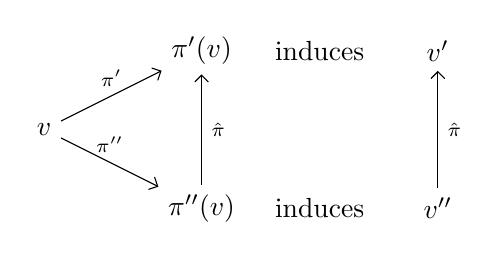
\begin{tikzpicture}[>= angle 90]
\draw (0,0) node (v) {$v$};
%
\draw (2,1) node (pi'v) {$\pi'(v)$};
\path[draw, ->] (v) -- node[above]{\scriptsize $\pi'$} (pi'v);
%
\draw (2,-1) node (pi''v) {$\pi''(v)$};
\path[draw, ->] (v) -- node[above]{\scriptsize $\pi''$} (pi''v);
\path[draw, ->] (pi''v) -- node[right]{\scriptsize $\hat\pi$} (pi'v);
%
\draw (pi'v)++(1.5,0) node (induces1) {induces};
\draw (induces1)++(1.5,0) node (v') {$v'$};
%
\draw (pi''v)++(1.5,0) node (induces2) {induces};
\draw (induces2)++(1.5,0) node (v'') {$v''$};
\path[draw, ->] (v'') -- node[right]{\scriptsize $\hat\pi$} (v');
\end{tikzpicture}
\end{center}
%
In fact, $\hat\pi$ will be the identity over all parameters except for fresh
parameters chosen under clause~\ref{clause:remap-4} of
Definition~\ref{def:representative-consistent-extension}.

We define $\pi''$ as an extension of~$\pi$.  This implies that $\pi''$
and~$\pi'$ agree on values in the domain of~$\pi$, and unify the same
components.  For all values~$y$ in the range of~$\pi$, we define $\hat\pi(y) =
y$. 

Recall that $v'.\fixed = v''.\fixed = post.\fixed$; each component of~$v'$ is
taken from~$post$ if the corresponding component of~$\pi'(v)$ is in~$pre$, and
otherwise is taken from~$\pi'(v)$; and each component of~$v''$ is taken
from~$post$ if the corresponding component of~$\pi''(v)$ is in~$pre$, and
otherwise is taken from~$\pi''(v)$.  We arrange for~$v'$ and~$v''$ to take the
same components from~$post$.

%% For each parameter~$x$ of~$v.\fixed$, we define $\pi''(x) = x$.  This means
%% $\pi''(v).\fixed = pre.fixed$.  And we define $\hat\pi(x) = x$. 

For each parameter~$x$ of~$v$ such that $y = \pi'(x)$ is a parameter of
$post.\fixed$, we define $\pi''(x) = y$, and $\hat\pi(y) = y$.  Note that each
such value~$y$ is included under case~\ref{clause:remap-1} of
Definition~\ref{def:representative-consistent-extension}.  This ensures
that~$\pi''(v)$ and~$\pi'(v)$ agree on all such~$y$; and hence~$v'$ and~$v''$
agree on all such~$y$.  Note that this is a consistent extension of~$\pi$,
because~$\pi'$ is a consistent extension of~$\pi$.  

For each parameter~$x$ such that $y = \pi'(x)$ is a parameter of a component
of~$v'$ taken from~$post$, we again define $\pi''(x) = y$, and $\hat\pi(y) =
y$.  Note that each such value $y$ is included under
case~\ref{clause:remap-2} or \ref{clause:remap-3} of
Definition~\ref{def:representative-consistent-extension}.  This ensures
that~$\pi''(v)$ and~$\pi'(v)$ agree on all such~$y$; and hence~$v'$ and~$v''$
agree on all such~$y$; in particular, they include the same components taken
from~$post$.  Again note that this is a consistent extension of~$\pi$,
because~$\pi'$ is a consistent extension of~$\pi$. 

Finally, each other parameter~$y$ in~$v'$ must necessarily be in a component
taken from~$\pi'(v)$.  Suppose the parameter is $\pi'(x)$, and $x$ is not in
the domain of~$\pi$.  We define $\pi''(x)$ to be the minimal fresh
parameter~$z$, chosen as in
Definition~\ref{def:representative-consistent-extension}; and we let
$\hat\pi(z) = y$.  This ensures that $v''$ uses~$z$ wherever $v'$ uses~$y$.
Also note that this is a consistent extension of~$\pi$, by construction.
\end{proof}

%%%%%

\begin{impNote}
\texttt{Unification.combine} produces the remapped version of~$v$, together
with information about the unifications.  If uses \texttt{allUnifs} to find
all choices of unification and corresponding renaming function~$\pi$.  Then
\texttt{extendUnif} extends this, and produces the remapped state.

\texttt{EffectOn.apply} produces the corresponding post-views.
\end{impNote}

%%%%%

\subsection{Optimisations} 


%%%%%

\begin{opt}
Recall Optimisation~\ref{opt:avoid-induced}.  
\begin{itemize}
\item For case~\ref{case:avoid-induced-1}, we avoid unifying the principal
  of~$v$ with the principal of~$pre$.

\item For case~\ref{case:avoid-induced-2}, if $pre.\fixed = post.\fixed$ we
  require that at least one component of~$v$ unifies with a component that
  changes state.

\item For case~\ref{case:avoid-induced-3}, we store a record of pairs
  $(v, post.\fixed)$ for which we have considered the effect of a transition
  $pre \trans{e} post$ on~$v$ for which $pre.\fixed \ne post.\fixed$,\,
  %% $unifs$ describes which components of~$v$ unify with which components
  %% of~$pre$ (
  and $v$
  unifies with no component.
%
  If subsequently we consider a similar case ---that is, the same
  $post.\fixed$ and~$v$, and no unifications--- we identify that it will not
  produce any new views, and so avoid the construction.
\end{itemize}
\end{opt}


\begin{impNote}
Done in isSufficientUnif. 
\end{impNote}

\begin{improve}
The third case is not quite the same as in
Optimisation~\ref{opt:avoid-induced}.  There we included cases where $pre$
and~$v$ shared a component that did not change state.  An obvious attempt to
implement this goes wrong: if there are two cases with the same $post.\fixed$
and~$v$, that include unifications of \emph{different} components that do not
change state, they might give different new views (with the unified components
having different parameters in $post.\fixed$).
%
For example
\begin{eqnarray*}
pre & = & (fixed; Th_1(T_0,N_0), Nd_A(N_0,N_1)) \\
post & = & (fixed'(N_1); Th_1'(T_0), Nd_A(N_0,N_1)) \\
v & = & (fixed; Th_v(T_0,N_0), Nd_A(N_0,N_1))
\end{eqnarray*}
unifying the two $Nd_A$ processes, with remapping $\set{T_0 \mapsto T_1, N_0
  \mapsto N_0,\linebreak[1] {N_1 \mapsto N_1}}$, induces
\[
(fixed'(N_1); Th_v(T_1,N_0), Nd_A(N_0,N_1) \equiv
(fixed'(N_0); Th_v(T_0,N_1), Nd_A(N_1,N_0)).
\]
But with 
\begin{eqnarray*}
pre' & = & (fixed; Th_2(T_0,N_0,N_1), Nd_A(N_0,N_2), Nd_N(N_1,Null)) \\
post' & = & (fixed'(N_1); Th_2'(T_0), Nd_A(N_0,N_2), Nd_N(N_1,Null))
\end{eqnarray*}
unifying the two $Nd_A$ processes, with remapping $\set{T_0 \mapsto T_1, N_0
  \mapsto N_0,\linebreak[1] {N_1 \mapsto N_2}}$, induces a transition to
\[\mit
(fixed'(N_1); Th_v(T_1,N_0), Nd_A(N_0,N_2)) \equiv
  (fixed'(N_0); Th_v(T_0,N_1), Nd_A(N_1, N_2)).
\]


If we have two cases concerning the same $post.\fixed$, $v$, and component~$c$
of~$v$ that unifies and doesn't change state, and $c$ unifies respectively
with~$c_1$ and~$c_2$ which differ only on parameters not in $post.\fixed$,
then it is enough to consider just one such case.  In the above example, we
had $c_1 = Nd_A(N_0,N_1)$,\, $c_2 = Nd_A(N_0,N_2)$ which differ on~$N_1$. 

\framebox{Do this.}  For the components, it's enough to store the list of
parameters shared with $post.\fixed$ and their indices. 
\end{improve}

 
%%%%%%%%%%%%%%%%%%%%

\begin{opt}
If the principal of~$v$ is unified with a component of~$pre$, and loses a
reference to a component~$c$, then all renamings of~$c$ produce the same final
view.  Thus it is enough to consider a single renaming, say the renaming that
agrees with the renaming within other components, but otherwise maps to fresh
parameters.  There is no need to explicitly construct the renaming of~$c$.  
%
\framebox{Consider this.}

This won't work with singleRef, however, because of cross references or
missing references. 
\end{opt}

%%%%%

\begin{improve} 
If the principal and another component~$c$ of~$v$ are both unified with
components of $pre$, and the principal of~$v$ loses the reference to~$c$ in
the transition, then for case~\ref{clause:remap-2} of
Definition~\ref{def:representative-consistent-extension}, we can ignore
parameters of~$c$.  This is only relevant for renaming of some third
component.
%
This might be useful when a node has a reference to the thread, but loses
that reference.
\end{improve}

%%% singleRef

\section{Views capturing a single reference}
\label{sec:singleRef}

In this section we consider the variation on our basic scheme, where each view
contains the state of only one secondary component referenced by the principal
(or none, if the principal references no component other than itself).  We
call these \emph{restricted views}, and use the term \emph{full views} for the
earlier version where we recorded all components referenced by the principal. 

We start by formalising restricted views.  Consider a system state~$s$, and a
particular component $cpt \in s.\cpts$.
\begin{itemize}
\item 
Suppose $cpt$ has no reference to another component.  Then we write $view(s,
cpt)$ for the view of the system state from~$cpt$, i.e.~the fixed processes
and $cpt$ itself.
\begin{eqnarray*}
view(s, cpt) & = &  (s.\fixed, \set{cpt}).
\end{eqnarray*}
This is the same as in the case of full views.

\item
Now suppose $cpt$ has $k > 1$ parameters (recall that its first parameter is
its own identity).  Suppose $1 < i \le k$ and $cpt.\params(i)$ is not a
distinguished value.  Then we write $view(s, cpt, i)$ for the view containing
$cpt$ and the state of the component referenced by its $i$th parameter.
\[
\begin{align}
view(s, cpt, i)  =  (s.\fixed, \set{cpt, c})\\ 
\mbox{where $c \in s.\cpt$ is such that $c.\id = cpt.\params(i)$}.
\end{align}
\]
\end{itemize}
%
We then define the set of views~$\V$ to be all such values:
%
\begin{eqnarray*}
\V & = & 
  \begin{align}
  \set{ view(s, cpt) \| s \in \S, cpt \in s.\cpts, \\
    \qquad   \mbox{$cpt$ has no reference to another component}} \union\null
  \\
  \set{ view(s, cpt, i) \| s \in \S, cpt \in s.\cpts, 
    1 < i \le length(cpt.\params), \\
    \qquad \mbox{$cpt.\params$ is not distinguished} }.
  \end{align}
\end{eqnarray*}

%%%%%%%%%%%%%%%%%%%%%%%%%%%%%%%%%%%%%%%%%%%%%%%%%%%%%%%

\subsection{Building abstract transitions}

We now consider how to adapt the constructions from the previous section so as
to build abstract transitions from such views.  Some of the changes we outline
are necessary for correctness; others are necessary to avoid false positives.

%% Note that if a transition represents a synchronisation between the principal
%% and a secondary component, we generate that only from the view that includes
%% that secondary component. (?)


We adapt the definition of a view transition to specify that if the principal
synchronises with one of the components that it references, then that
secondary component must be included in the view transition.  The definition
of an extended transition is then as earlier. 
%
\begin{definition}
\label{def:active-process-transition-singleRef}
We define a \emph{view transition} of view~$v$ to be a transition $v \trans{e}
v'$ such that
%
\begin{itemize}
\item $v$ has either an active principal or an active fixed process with $e$
  in its alphabet;

\item If $v.\princ$ has a reference to a component with $e$ in its alphabet,
  then $v$ contains such a component;

\item $v'$ is the same as~$v$ except replacing every (fixed or component)
  process~$p$ that has $e$ in its alphabet with a process $p'$ such that \( p
  \trans{e} p' \).
\end{itemize}

Given a view transition $v \trans{e} v'$, we define the corresponding
\emph{extended transitions} $pre \trans{e} post$,  as in
Definition~\ref{def:active-process-transition}.  Finally, we extract views of
the principal component.  
\end{definition}


For example, consider the following view transition using full
views, as in the previous section.
%
\begin{equation}
\begin{align}
\label{trans:setNext}
(fixed; Th(t, n, n'), Nd_x(n, null), Nd_y(n', n'')) 
  \trans{setNext.t.n.n'} \\
\qquad (fixed'; Th'(t, n, n'), Nd_x(n, n'), Nd_y(n', n'')).
\end{align}
\end{equation}
%
When we use restricted views, we would include the following view transition,
which contains the node~$n$ that synchronises on the transition. 
%
\begin{equation}
\label{trans:setNext-singleRef}
\begin{align}
(fixed; Th(t, n, n'), Nd_x(n, null)) 
  \trans{setNext.t.n.n'} \\
\qquad (fixed'; Th'(t, n, n'), Nd_x(n, n')).
\end{align}
\end{equation}
%
However we do not consider a view transition from
\[\mit
(fixed; Th(t, n, n'), Nd_y(n', n'')), 
\]
because that view does not contain a component for~$n$, which synchronises on
the transition.  Instead, such transitions are induced: see
Section~\ref{sec:singleRef-induced}. 

\begin{impNote}
\texttt{system.transitions} suppresses transitions that involve a
synchronisation with a missing component.
\end{impNote}

%%%%%%%%%%%%%%%%%%%%%%%%%%%%%%%%%%%%%%%%%%%%%%%%%%%%%%%
 % Definition and start of transitions
\subsection{Induced transitions}
\label{sec:singleRef-induced}

We now consider how to adapt the definition of induced transitions.  This
subsumes a fairly obvious adaptation of
Definition~\ref{def:induced-transition}.  For example, the
transition~(\ref{trans:setNext-singleRef}) induces a transition on
\[\mit
v = (fixed; Thread(t, n, n'), Node_y(n', n''))
\]
to produce
\[\mit
v' = (fixed'; Thread'(t, n, n'), Node_y(n', n'')). 
\]
Thus omitting view transitions from~$v$ (as discussed above) does not prevent
us producing~$v'$. 

However, it turns out that we need to:
\begin{enumerate}
\item consider another form of induced transitions, concerning secondary
  components from the extended transition; and

\item enforce extra conditions for induced transitions, in order to avoid our
  algorithm discovering certain false errors.
\end{enumerate}
%
We discuss point~1 next; we then give our revised definition of induced
transitions; and then justify the extra conditions mentioned in point~2.

%%%%%%%%%%%%%%%%%%%%%%%%%%%%%%%%%%%%%%%%%%%%%%%%%%%%%%%

\subsubsection{Secondary induced transitions}
\label{ssec:c2Refs}

%% However, we need an additional mechanism to capture some extra views that
%% would otherwise be missed, in particular  where a secondary
%% component gains a reference to another component.  

Consider again the transition (\ref{trans:setNext}).  When using full views,
this would induce a transition from 
\[\mit
v = (fixed,  Node_x(n, null))\]
to produce
\[\mit
v' = (fixed';  Node_x(n, n'), Node_y(n', n'')).
\]
However, with restricted views and a direct adaptation of
Definition~\ref{def:induced-transition}, no corresponding transition
producing~$v'$ via transition~(\ref{trans:setNext-singleRef}) is induced,
because the component state $Node_y(n', n'')$ is in neither~$v$ nor the
post-state of the view transition.

Instead, we consider the effect of the 
transition~(\ref{trans:setNext-singleRef}) on views such as
\[\mit
v = (fixed; Node_y(n', n''), Node_z(n'', n''')).
\]
We identify that the secondary component in the  transition gains a
reference to the principal node of~$v$, and use that to deduce the induced
transition. 

More generally, consider an extended transition $pre \trans{e} post$ and a
view $v$ such that $v$ and $pre$ are accordant, and such that a secondary
component~$sc$ of~$post$ has a reference to $v.\princ$.  Then (subject to some
extra conditions that we describe below) the transition induces a new
transition producing
\[\mit
v' = (post.\fixed, \set{sc, v.\princ}).
\]

\begin{impNote}
At present this is done in EffectOn, via c2Refs. 
\end{impNote}

\begin{improve}
I don't think this is the
best way.  I think that we want to separately record that for every view
\[\mit 
(\fixed; Thread(t, n, n'), Node_y(n', n''))
\]
we generate the view~$v'$ (for all $y$ and~$n''$).  More generally, if a
secondary component changes state, and gains a reference to a missing
secondary component, then we create an appropriate record.
\end{improve}


%%%%%%%%%%%%%%%%%%%%%%%%%%%%%%%%%%%%%%%%%%%%%%%%%%%%%%%

\subsubsection{Definition of induced transitions}

We now adapt Definition~\ref{def:induced-transition} to describe how
transitions are induced for restricted views.  We justify conditions~(b)
and~(c) of the following definition in Sections~\ref{ssec:cross-refs}
and~\ref{ssec:missing-common}, respectively.  The first form of induced
transition is analogous to Definition~\ref{def:induced-transition} (the only
change is in clause~\ref{induce-clause-3}).  The second form is as discussed
in Section~\ref{ssec:c2Refs}.
%
\begin{definition}
\label{def:induced-transition-singleRef}
Consider an extended transition~$pre \trans{e} post$, and a view $v \in V$
such that:
%
\begin{enumerate}
\item[(a)] $v$ and $pre$ are accordant;

\item[(b)] If a component $c$ of $pre$ has a reference
  to a component~$c'$ of~$v$, or vice versa, then $V$ also contains the view
\begin{eqnarray*}
v_\cross & = & (pre.\fixed, \set{c, c'});
\end{eqnarray*}

\item[(c)] If the principals of~$pre$ and~$v$ both have a reference to the
  same missing component, say with identity $id$, then there is some
  component~$c$ with identity~$id$ such that $V$ contains each of
\[
(pre.\fixed, \set{pre.\princ, c}) \quad\mbox{and}\quad 
(v.\fixed, \set{v.\princ, c})
\]
(recall $pre.\fixed = v.\fixed$ here).
\end{enumerate}
%
Then the transition \emph{induces} a new
transition $v \trans{} v'$ where
\begin{enumerate}
\item $v'.\fixed = post.\fixed$.

\item If $v.\princ$ is in $pre$ then $v'.\princ$ is the corresponding
  component in~$post$; otherwise $v'.\princ = v.\princ$.

\item\label{induce-clause-3} If $v'.\princ$ has no reference to another
  component, then $v'$ has no secondary component.  Otherwise the secondary
  component of~$v'$ is a component referenced by $v'.princ$, either from
  $post$ if the component is part of the transition, or otherwise from~$v$, if
  such a component exists.  If $v'.\princ$ references only components not in
  either $post$ or $v$, then no new transition is induced.
\end{enumerate}
%
Further, if a secondary component~$sc$ of~$post$ has a reference to $v.\princ$,
then the transition induces a new transition producing
\[\mit
v' = (post.\fixed, \set{sc, v.\princ}).
\]
\end{definition}

\begin{improve}
Can we reduce the number of combinations we have to consider?
At present we don't support Optimisation~\ref{opt:avoid-induced} with reduced
views: it's not sound for some reason.  Work out why.  It might be due to the
use of c2Refs.
\end{improve}


%%%%%%%%%%%%%%%%%%%%%%%%%%%%%%%%%%%%%%%%%%%%%%%%%%%%%%%

\subsubsection{Compatible cross references}
\label{ssec:cross-refs}

We now justify condition~(b) from
Definition~\ref{def:induced-transition-singleRef}, that if a component~$c$
of~$pre$ has a reference to a component~$c'$ of~$v$, or vice versa, then $V$
must also contain the view
\begin{eqnarray*}
v_\cross & = & (pre.\fixed, \set{c, c'}).
\end{eqnarray*} 
In effect, this requires cross references between $c$ and~$pre$ to be
represented by other views.  If $c$ and $pre$ are views of the same system
state, then the view $v_X$ will also be a view of that state; hence requiring
it is sound.
%
We give two examples to show why not requiring the compatibility of cross
references can lead to the discovery of false errors. 

Consider the following transition for the lock-based queue.
\[
\begin{align}
(fixed(t, n_1, n_1); Enq_5(t, n_1, n_2), Nd_B(n_2, null)) 
  \trans{setLast.t.n_2} \\
\qquad (fixed(t, n_1, n_2); Enq_6(t), Nd_B(n_2, null)).
\end{align}
\]
The thread is enqueueing~$B$ in node~$n_2$.  It has previously set $n_1$ to
point to $n_2$, and now advances \SCALA{last} to~$n_2$.  This implies that
$n_1$ is of the form $Nd_x(n_1, n_2)$ for some~$x$ in any corresponding system
state.  However, consider also the view
%
\begin{eqnarray*}
v & = & (fixed(t, n_1, n_1) ; Nd_A(n_1, null)).
\end{eqnarray*}
This is accordant with the pre-state of the transition; so, without
condition~(b), a transition to
\begin{eqnarray*}
v' & = & (fixed(t, n_1, n_2) ; Nd_A(n_1, null))
\end{eqnarray*}
would be induced.  But now a subsequent pop would find the stack empty (since
$n_1$ is the dummy header node and has a null next reference), despite the
previous push.  (In section~\ref{sec:???}, we will consider this example
together with a watchdog that expects a single~$B$ to be pushed, and signals
an error if a thread finds the stack empty when it should contain~$B$; thus
the watchdog would falsely signal an error here.)

Condition~(b) of Definition~\ref{def:induced-transition-singleRef} would
require the existence of a view
\begin{eqnarray*}
v_\cross & = & (fixed(t, n_1, n_1); Enq_5(t, n_1, n_2), Nd_A(n_1, null)),
\end{eqnarray*}
in order to induce the transition that produces~$v'$, because the enqueueing
thread has a (missing) reference to~$n_1$.  However, no such view exists in
the model (since the thread is in a state where it has just updated~$n_1$ to
point to~$n_2$).  Hence condition~(b) prevents the false error.

%%%%%

The previous example showed that it is necessary to consider cross references
from a principal.  The following example shows that it is also necessary to
consider cross references from a secondary component.  

In Section~\ref{sec:lock-based-stack} we will consider a lock-based stack.
There, for the purposes of specification, we will ensure that if the value~$B$
is in the stack, all values below it in the stack equal~$A$, and all values
above it equal~$C$.  We will include a watchdog that, when $B$ is in the
stack, does not allow a pop of~$A$.  (We justify this watchdog in
Section~\ref{sec:lock-based-stack}.) 

Consider the transition
\[
\begin{align}
(Top(n_1), WD_B ; Pop(t, n_1, n_2), Nd_C(n_1, n_2)) \trans{setTop.t.n_2} \\
\qquad  (Top(n_2), WD_B ; Pop'(t), Nd_C(n_1, n_2)) .
\end{align}
\]
The thread is popping $C$ from the node~$n_1$.  It advances the
\SCALA{top} variable to the next node~$n_2$.  Here $WD_B$ is the watchdog, in
a state where $B$ is in the stack.  

Consider also the view
\begin{eqnarray*}
v & = & (Top(n_1), WD_B ;  Nd_A(n_2, null)).
\end{eqnarray*}
This is accordant with the pre-state of the transition (and consistent with a
system state where $n_2$ is at the bottom of the stack, below the $B$-node).
Hence, without condition~(b), a transition to
\begin{eqnarray*}
v' & = & (Top(n_2), WD_B ;  Nd_A(n_2, null)).
\end{eqnarray*}
would be induced.  But now a subsequent pop would obtain~$A$.  At this point
the watchdog would give an error: it does not allow $A$ to be popped when $B$
is in the stack.

With the addition of condition~(b), we would require the existence of the view
\begin{eqnarray*}
v_\cross & = &  (Top(n_1), WD_B ; Nd_C(n_1, n_2), Nd_A(n_2, null)).
\end{eqnarray*}
%
However, no such view exists in the model: it is an invariant of the model
that a $C$ node never points to an~$A$ node.  This prevents the false error.

%% consistent with $pre$, so induces transition to
%% \[
%% (Top(n_2), WD_B ;  Nd_A(n_2, null)
%% \]
%% so subsequent pop gets A.


%%%%%%%%%%%%%%%%%%%%%%%%%%%%%%%%%%%%%%%%%%%%%%%%%%%%%%%

\subsubsection{Checking consistent common missing components}
\label{ssec:missing-common}

We now justify condition~(c) from
Definition~\ref{def:induced-transition-singleRef}, that if the principals
of~$pre$ and~$v$ both have a reference to the same missing component, say with
identity $id$, then there must be some component~$c$ with identity~$id$ such
that $V$ contains each of
\[
(pre.\fixed, \set{pre.\princ, c}) \quad\mbox{and}\quad 
(v.\fixed, \set{v.\princ, c}).
\]
In other words, there is some way of consistently instantiating the missing
component~$c$ that is common to both views. When using full views,
$c$ would have been included in both substates, and so the check would have
been included within Definition~\ref{def:induced-transition}.

%% Consider transitions induced on view~$v$ by an extended transition $pre
%% \trans{e} post$.  In particular, consider the case where the principals in
%% $pre$ and $v$ both have a missing reference to the same component~$c$.  It
%% turns out that it is necessary to check that there is a state for the missing
%% component~$c$, consistent with both~$pre$ and~$v$.  (When using full views,
%% $c$ would have been included in both substates, and so the check would have
%% been included within Definition~\ref{def:induced-transition}.)


We explain the necessity using an example from the Treiber
Stack~\cite{treiber}, which we will discuss in Section~\ref{sec:treiber}.  In
that section, in order to capture the correctness condition of being a stack,
we arrange for the stack to hold at most a single node containing~$B$, and for
all nodes below it in the stack to contain~$A$; the correctness conditions
include that~$B$ is popped at most once.

%%%%%

\begin{figure}\small
% Add a label with text #2 just above #1
\def\addLabel#1#2{\draw #1++(0,0.5) node {#2};}
\begin{center}
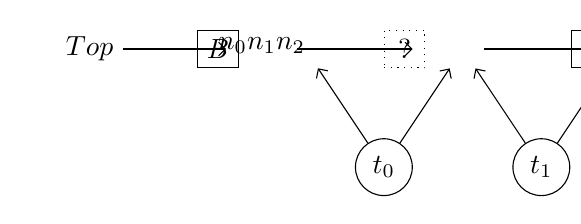
\begin{tikzpicture}[>= angle 90]
\draw (0,0) node[draw] (n0) {$B$}; \addLabel{(n0)}{$n_0$}
\draw (n0) ++ (-2,0) node (top) {$Top$}; \draw[->] (top) -- (n0);
\draw (n0) ++ (2,0) node[draw,dotted] (n1) {$\,?\,$}; \addLabel{(n1)}{$n_1$}
\draw[->] (n0) -- (n1);
\draw (n1) ++ (2,0) node[draw] (n2) {$A$}; \addLabel{(n2)}{$n_2$}
\draw[->] (n1) -- (n2);
%%% threads
\draw (n0) ++ (1,-1.5) node[draw,circle] (t0) {$t_0$};
\draw[->] (t0) -- (n0); \draw[->] (t0) -- (n1);
\draw (n1) ++ (1,-1.5) node[draw,circle] (t1) {$t_1$};
\draw[->] (t1) -- (n1); \draw[->] (t1) -- (n2);
\end{tikzpicture}
\end{center}
\caption{Illustration of a scenario from the Treiber Stack.  Nodes are
  depicted in rectangular boxes, and threads in circles.}
\label{fig:missingCommon}
\end{figure}

%%%%%

Consider the following two views
%
\begin{eqnarray*}
pre & = &  (Top(n_0), WD_B; Thread_{pop,B}(t_0, n_0, n_1), Nd_B(n_0, n_1)), \\
v & = & (Top(n_0), WD_B; Thread_{pop,B}(t_1, n_1, n_2), Nd_A(n_2, null)).
\end{eqnarray*}
%
These are depicted in Figure~\ref{fig:missingCommon}.  Both principals are
threads that are attempting to perform a pop, of nodes~$n_0$ and~$n_1$,
respectively, each having read~$B$ from that node.  Both views have an omitted
reference to node~$n_1$, depicted as dotted in the figure.  Both are possible
views of the system, but they are not consistent.

From the state $pre$, thread~$t_0$ can advance \SCALA{top} to~$n_1$,
popping~$B$, in a transition that produces
\[\mit
(Top(n_1); Thread(t_0), Nd_B(n_0, n_1)).
\]
Without condition~(c), this transition  induces a transition from~$v$ to
\[\mit
(Top(n_1); Thread_{pop,B}(t_1, n_1, n_2), Nd_A(n_2, null)).
\]
But now $t_1$ can pop~$B$ (from~$n_1$).  The watchdog will then falsely signal
an error (since it has seen~$B$ popped twice). 

Including condition~(c) will prevent this false error, since there is no state
for~$n_1$ that is consistent with the states of both~$t_0$ and~$t_1$.
Thread~$t_0$ is in a state that is consistent only with~$n_1$ holding~$A$ (it
is an invariant of the model that a $B$-node can point only to an $A$-node);
and $t_1$ is in a state that is consistent only with~$n_1$ holding~$B$.

%% Without condition~(c), the analysis finds a false error: $t_0$ pops~$B$
%% (from~$n_0$), advancing $Top$ to~$n_1$; and then $t_1$ also pops~$B$
%% (from~$n_1$).

%% In order to avoid false positives like this, we identify if the principals of
%% the two views~$pre$ and~$v$ both have a reference to the same missing
%% component, say with identity $id$.  If so, we search the set of views~$V$ to
%% try to identify a component~$c$ with identity~$id$ such that each of
%% \[
%% (pre.\fixed, \set{pre.\princ, c}) \quad\mbox{and}\quad 
%% (v.\fixed, \set{v.\princ, c}
%% \]
%% are in $V$ (recall $pre.\fixed = v.\fixed$ here). 

\begin{impNote}
This is done in \texttt{EffectOn.\linebreak[1]check\-Compatible\-Missing}.  To
fit with breadth-first search, if there is no way to instantiate the common
missing component, we store relevant information in \texttt{EffectOnStore} in
case relevant views are found subsequently.
\end{impNote}
 % induced transitions


%%%%%%%%%%%%%%%%%%%%%%%%%%%%%%%%%%%%%%%%%%%%%%%%%%%%%%%

\subsection{Correctness}

Formalise procedure.

\begin{lemma}
Let $V$ be a set of views.  Every abstract transition from~$V$ is generated by
the procedure in Definition~\ref{???}.
\end{lemma}

\begin{proof}
Consider an abstract transition
\[
\gamma(V) \ni s \trans{e} s' \sqge_{\V} v'.
\]
We need to show that we generate $v'$ as part of the process described above.

Let $fixed = s.\fixed$ and $fixed' = s'.\fixed$.  

Consider a corresponding extended transition $pre \trans{e} post$, i.e.~such
that: $pre.\fixed = fixed$,\, $post.\fixed = fixed'$; the principal of $pre$
and $post$ is the active component of the concrete transition; if another
component to which the principal has a reference synchronises on the
transition, then that is included in~$pre$ and $post$ (otherwise choose an
arbitrary view of the principal); and $pre$ and~$post$ also include any other
component relevant to the transition (i.e.~that synchronises on the transition
or to which the principal gains a reference).

\framebox{active fixed component}

Let $pId = v'.\princ.id$ be the identity of the principal of~$v'$, and suppose
that component has states $princ$ and $princ'$ in~$s$ and~$s'$, respectively
(so $princ \trans{e} princ'$).

\begin{enumerate}
\item First suppose that $pId$ is the active component in the concrete
  transition $s \trans{e} s'$, and so in the extended transition $pre
  \trans{e} post$.  And suppose that either (a)~no other component
  synchronises on the transition, or (b)~that another component does
  synchronise and is included in~$v'$, or (c)~that the principal gains a
  reference to another component in the transition, and that component is
  included in~$v'$.  In each case, the extended transition captures the
  relevant information, and so $v'$ can be extracted from~$post$.

\item Now suppose again that $pId$ is the active component in the concrete
  transition $s \trans{e} s'$, but that the secondary component~$c$ in~$v'$ is
  not in the corresponding extended transition (as in the previous case).
  Then necessarily $pId$ had a reference to~$c$ in~$s$, and $c$ did not change
  state in the transition.  Let $v = (fixed, \set{princ, c})$.  Then the
  transition $v \trans{} v'$ is induced, as in Definition\ref{def:induced-transition}

??????????

\end{enumerate}

\end{proof}
 % correctness
\subsection{Identifying sufficient remappings}

\framebox{Introduce} term \emph{linkage} earlier.

\framebox{*** combine this with the next subsection}  Arguably some of this
should be covered when considering full views. 

In this section we consider the problem of calculating all induced transitions
produced by a transition $pre \trans{} post$ acting on view~$v$, given that
both are represented in normal form.  We want to produce all resulting views
corresponding to the transition acting on a remapping of~$v$, up to
equivalence.  Our aim, then, is to identify sufficient remappings to guarantee
this.  But, in the interests of efficiency, we want to avoid considering too
many remappings.  The necessity of considering linkages complicates the
process over that for full views.

%% Having to deal with linkages when considering induced transitions adds
%% considerable cost to the checking procedure.  In this section we show that it
%% is sound to omit certain renamings of a view~$v$ when considering the effects
%% of a transition on it: we show that in such cases equivalent views can be
%% produced by induced transitions from a different renaming.  

There are two facets to consider.
%
\begin{enumerate}
\item Two different remappings of the view~$v$ may lead to equivalent views
  being produced by the induced transition (on the assumption that
  conditions~(b) and~(c) are satisfied in each case).

\item Tho different remappings of~$v$ that lead to equivalent views may
  require different views to satisfy conditions~(b) and~(c).  When these
  required views are unrelated, we need to consider both remappings.  However,
  in some cases, the required views for one remapping may be a proper subset
  of those for the other remapping (up to equivalence); in this case it is
  sound, and more efficient, to consider just the former.  
\end{enumerate}

Our approach is as follows.  We build up each remapping function in stages; in
early stages, the remapping will be a partial function, that is gradually
extended to give values for all parameters of the view~$v$. 
\begin{itemize}
\item We start with a partial unification function~$\pi_u$. 

\item We then extend $\pi_u$ in all ways that will lead to distinct resulting
  views (cf.~item~1 above).  For each distinct resulting view (up to
  equivalence), we define a single extension that will produce it.  We call
  each such extension a \emph{result-defining remapping}.  Each is a partial
  function, extending $\pi_u$ over those parameters that are necessary to
  define the result.  
  We describe our approach in Sections~\ref{sec:primary-result-defining}
  and~\ref{sec:secondary-result-defining} for primary- and secondary-induced
  transitions, respectively.

\item We then consider conditions~(b) and~(c) of
  Definition~\ref{def:induced-transition-singleRef}.  For each result-defining
  remapping, we consider different extensions that will correspond to
  different required views, but omitting a remappings that requires a
  proper superset of those for another (cf.~item~2 above).  
  We consider conditions~(b) and~(c) in Sections~\ref{sec:necessary-b}
  and~\ref{sec:necessary-c}, respectively, proving appropriate results.  We
  then present and prove our algorithm for calculating sufficient
  remappings in Section~\ref{sec:necessary-algorithm}.

\end{itemize}

We fix a transition $pre \trans{} post$ and a view~$v$ for the remainder of
this section. 


%%%%%%%%%%%%%%%%%%%%%%%%%%%%%%%%%%%%%%%%%%%%%%%%%%%%%%%

\subsubsection{Remappings for equivalent primary induced transitions}
\label{sec:primary-result-defining}

We start by considering when two different extensions of the same partial
unification function produce equivalent primary induced views.  The following
examples help to illustrate. 

\begin{example}\label{example:29}
Consider the normal-form transition
\begin{eqnarray*}
(fixed(N_0); Th(T_0,N_1), Nd_A(N_1,N_2)) & \trans{} &
  (fixed'(N_0); Th'(T_0,N_1), Nd_A(N_1,N_2))
\end{eqnarray*}
acting on 
\[
(fixed(N_0); Nd_B(N_1,N_2), Nd_C(N_2,N_3)).
\]
No unification is possible, so the only unification function is $\pi_{u} =
\set{N_0 \mapsto N_0}$.  If we consider the mapping $\pi_1 = \set{N_0 \mapsto
  N_0, \linebreak[1] {N_1 \mapsto N_3,} \linebreak[1] {N_2 \mapsto N_4},
  \linebreak[1] N_3 \mapsto N_5}$ (mapping all parameters other than those in
the fixed processes to fresh values), then this induces a transition to
\[
(fixed'(N_0); Nd_B(N_3,N_4), Nd_C(N_4,N_5)) \equiv 
  (fixed'(N_0); Nd_B(N_1,N_2), Nd_C(N_2,N_3)).
\] 

Consider instead the mapping $\pi_2 = \set{N_0 \mapsto N_0, N_1 \mapsto N_3,
  N_2 \mapsto N_4,\linebreak[1] {N_3 \mapsto N_1}}$.  This mapping produces a
linkage that would require a view equivalent to $v_\cross = (fixed(N_0);
Nd_C(N_4,N_1), Nd_A(N_1,N_2))$.  If such a view exists, the induced transition
produces
\[
(fixed'(N_0); Nd_B(N_3,N_4), Nd_C(N_4,N_1)) \equiv 
  (fixed'(N_0); Nd_B(N_1,N_2), Nd_C(N_2,N_3)).
\]
The two mappings produce equivalent views.  Thus it is enough to consider one
of them.  We consider only the mapping~$\pi_1$, as it subsumes~$\pi_2$, and is
simpler to deal with as it does not require the additional view equivalent
to~$v_\cross$.

The same is true of all other remappings with $N_1$ and/or $N_2$ in the range
(there are seven in total).
\end{example}

%%%%%

The following example shows how different remappings can produce
non-equivalent views.
% 
\begin{example}\label{example:singleRef-remapping-post-servers}
Consider the transition
% 
\begin{eqnarray*}
(fixed(N_0); Th(T_0,N_1), Nd_A(N_1,N_2)) & \trans{} &
  (fixed'(N_1); Th'(T_0,N_1), Nd_A(N_1,N_2))
\end{eqnarray*}
acting on
\[
v = (fixed(N_0); Nd_B(N_1,N_2), Nd_C(N_2,N_3)).
\]
Again no unification is possible.  The remapping function $\pi_1 = \set{N_0
  \mapsto N_0, \linebreak[1] {N_1 \mapsto N_3}, \linebreak[1] {N_2 \mapsto
    N_4}, \linebreak[1] {N_3 \mapsto N_5}}$ induces a transition to
\[
(fixed'(N_1); Nd_B(N_3,N_4), Nd_C(N_4,N_5)) \equiv
(fixed'(N_0); Nd_B(N_1,N_2), Nd_C(N_2,N_3)).
\]

Alternatively, the remapping function $\pi_2 = \set{{N_0 \mapsto N_0}, {N_1
    \mapsto N_3}, \linebreak[1] {N_2 \mapsto N_4}, \linebreak[1] {N_3 \mapsto
    N_1}}$ creates a linkage via~$N_1$, requiring a view equivalent to
$(fixed(N_0); Nd_C(N_4,N_1), Nd_A(N_1,N_2))$.  If such a view does exist, the
induced transition produces
\[
(fixed'(N_1); Nd_B(N_3,N_4), Nd_C(N_4,N_1)) \equiv
(fixed'(N_0); Nd_B(N_1,N_2), Nd_C(N_2,N_0)).
\]
This is not equivalent to the view produced previously.  Thus it is necessary
to consider both unification functions.

The critical point is that $\pi_2$ maps~$N_3$ to a value in $post.\fixed$,
which leads to a different induced view to that for $\pi_1$.

Note that neither~$N_1$ nor~$N_2$ can be mapped to~$N_1$, since this would
require a unification of components. 
\end{example}

%%%%%

We now give sufficient conditions for two induced transitions to produce
equivalent views, on the assumption that conditions~(b) and~(c) of
Definition~\ref{def:induced-transition-singleRef} are satisfied. 
We say that two remapping functions~$\pi_1$ and~$\pi_2$ \emph{range-agree}
on~$y$ if they map the same variables to~$y$:
\[
\forall x \spot \pi_1(x) = y \iff \pi_2(x) = y.
\]
Necessarily there is at most one~$x$ that the remapping functions map
to~$y$.

\begin{definition}
Consider a transition $pre \trans{} post$ and a view~$v$, both in normal form.
Consider a partial unification function~$\pi_u$.  We define the
\emph{result-relevant parameters} to be:
%
\begin{enumerate}
\item\label{item:singleRef:remappings-equivalent:post-servers} All parameters
  of $post.\fixed$;

\item For each component~$c$ of~$v$ that is unified with a component of~$pre$,
  all new parameters gained by~$c$ in the transition;

\item If the principal of~$v$ is unified with a component of~$pre$, and
  acquires a reference to a component~$c'$ of~$post$, then all parameters
  of~$c'$. 
\end{enumerate}
\end{definition}

\begin{lemma}
\label{lem:singleRef:remappings-equivalent-primary}
Consider a transition $pre \trans{} post$ and a view~$v$, both in normal form.
Consider a partial unification function~$\pi_u$, and two consistent
extensions~$\pi_1$ and~$\pi_2$, and suppose that $\pi_1$ and $\pi_2$
range-agree on all result-relevant parameters.  Let $v_1 = \pi_1(v)$ and $v_2
= \pi_2(v)$.  Suppose, further, that conditions~(b) and~(c) of
Definition~\ref{def:induced-transition-singleRef} are satisfied for the
induced transitions from~$v_1$ and~$v_2$.  Then for each view~$v_1'$ produced
by a primary induced transition from~$v_1$, there is a view~$v_2'$ produced by
a primary induced transition from~$v_2$, such that $v_1' \equiv v_2'$; and
vice versa.
\end{lemma}

%%%%%

\framebox{**} Discussion of examples.
Example~\ref{example:singleRef-remapping-post-servers} illustrates
item~\ref{item:singleRef:remappings-equivalent:post-servers}.  Examples to
illustrate other aspects. 

%%%%%

\begin{proof}
Consider a particular view~$v_1'$ produced by a primary induced transition
from~$v_1$.  Let $v_2'$ be the corresponding view produced by a primary
induced transition from~$v_2$, i.e.~if the secondary component of~$v_1'$ (if
any) corresponds to the $k$th reference of~$v_1'.\princ$, then the secondary
component of~$v_2'$ corresponds to the $k$th reference of~$v_2'.\princ$.

Note that if the principals of $v_1$ and~$v_2$ are unified with a component
of~$pre$ (necessarily the same component in each case), the principals of the
induced views are the corresponding components of~$post$ (so equal).
Otherwise, the principals of the induced views are the principals of~$v_1$
and~$v_2$, respectively. 

Concerning secondary components, note that one of the following holds:
%
\begin{itemize}
\item The secondary components of~$v_1'$ and~$v_2'$ are the same component
  of~$post$; 

\item The secondary components of~$v_1'$ and~$v_2'$ are, respectively, the
  secondary components of~$v_1$ and~$v_2$, which were not unified with a
  component of~$pre$; or

\item Neither has a secondary component.
\end{itemize}

This implies that $v_1'$ and~$v_2'$ agree on all parameters of~$post.\fixed$,
and all parameters of components that were taken from~$post$, by the three
cases in the definition of result-relevant parameters.  All other parameters
are only in components taken from~$v_1$ or~$v_2$, respectively, that did not
unify with any component and so did not change state in the transition; the
parameters will be $\pi_1(x)$ and~$\pi_2(x)$, respectively, where $x$ is the
corresponding parameter of~$v$.  Thus $v_1' \equiv v_2'$.
\end{proof}

Optimisation: I think we don't need to agree on parameters of the secondary
component if that isn't included in the subsequent view.  That means qualify
condition~(2) of the lemma with: ``if $c$ is a secondary component of~$v$,
then the principal of~$v$ does not lose the reference to~$c$.''  This is an
issue only if both components of~$v$ change state, which is quite rare.

%%%%%

\begin{definition}
Consider a partial unification function~$\pi_u$.  We call a partial consistent
extension~$\pi_{rd}$ a \emph{minimal primary-result-defining remapping} if all
values in the range of~$\pi_{rd}$ that are not in the range of~$\pi_u$ are
result-relevant parameters.

We say a consistent extension~$\pi$ of~$\pi_{rd}$ is a
\emph{result-consistent} extension if it adds no new result-relevant
parameters to the range.  We will also sometimes say that $\pi$ is a (not
necessarily minimal) primary-result-defining remapping.
\end{definition}

%%%%%

\begin{example}
Consider again the processes of
Example~\ref{example:singleRef-remapping-post-servers}.  The unification
function $\pi_u = \set{N_0 \mapsto N_0}$ has minimal primary-result-defining
remappings $\pi_u$ itself and $\pi_u \union \set{N_2 \mapsto N_1}$.  Each
result-consistent extension of one of these will map no other parameter
to~$N_1$. 
\end{example}


%% For instance, in Example \ref{example:29}, the extension $\set{N_0
%%   \mapsto N_0, \linebreak[1] {N_3 \mapsto N_1}}$ of $\set{N_0 \mapsto N_0}$ is
%% result-defining since $N_1$ corresponds to the first case of
%% Lemma~\ref{lem:singleRef:remappings-equivalent-primary}. 

The following corollary shows that all result-consistent extensions of a
primary-result-defining remapping produce the same resulting view (up to
equivalence); it follows immediately from
Lemma~\ref{lem:singleRef:remappings-equivalent-primary}.
%
\begin{corollary}
Let $\pi_{rd}$ be a (not necessarily minimal) primary-result-defining
remapping.  Let $\pi_1$ and~$\pi_2$ be two result-consistent extensions
of~$\pi_{rd}$.  Let $v_1 = \pi_1(v)$ and $v_2 = \pi_2(v)$.  Suppose
conditions~(b) and~(c) of Definition~\ref{def:induced-transition-singleRef}
are satisfied for~$v_1$ and~$v_2$.  Then for each view~$v_1'$ produced by a
primary induced transition from~$v_1$, there is a view~$v_2'$ produced by a
primary induced transition from~$v_2$, such that $v_1' \equiv v_2'$; and vice
versa.
\end{corollary}

\framebox{***} does the implementation consider only result-consistent
extensions? 

%%%%%%%%%%%%%%%%%%%%%%%%%%%%%%%%%%%%%%%%%%%%%%%%%%%%%%%


\subsubsection{Remappings for equivalent secondary induced transitions}
\label{sec:secondary-result-defining}

We now consider secondary induced transitions. 
% 
\begin{definition}
Let $\pi_u$ be a unification function.  Suppose $x$ is a parameter of some
secondary component~$sc$ of $post$,  of the same type as
$v.\princ.\id$, and such that $sc$ acquires that reference~$x$ in the
transition.  Consider $\pi_{rfd} = \pi_u \union \set{v.\princ.\id \mapsto x}$, and
suppose this is a consistent extension: so either
\begin{itemize}
\item $(v.\princ.\id \mapsto x) \in \pi_u$; or
\item $v.\princ.\id \nin \dom \pi_u$,\, $x \nin \ran \pi_u$, and $x$ is not
  the identity of a component in~$pre$ and $post$.
\end{itemize}
%
Then we say that $\pi_{rfd}$ is a \emph{secondary-reference-defining}
function.  Note that it creates a reference from~$sc$ to the renamed principal
of~$v$.
\end{definition}

%%%%%
%% Let $\pi_{rd}$ be a consistent extension of~$\pi_1$, adding mappings for
%% parameters of~$v.\princ$ (if necessary).  Then we say that $\pi_{rd}$ is a
%% \emph{secondary-result-defining function}.  This remapping corresponds to a
%% secondary induced transition that produces $(post.\fixed; \set{sc,
%%   \pi_{rd}(v.\princ)})$.

\begin{definition}
Consider a transition $pre \trans{} post$ and a view~$v$, both in normal form.
Consider a secondary-reference-defining function~$\pi_{rfd}$ corresponding to
secondary component~$sc$ acquiring a reference to~$v.\princ$.  We define the
\emph{result-relevant parameters} to be all parameters of $post.\fixed$
and~$sc$.
\end{definition}

%%%%%

\begin{lemma}
\label{lem:singleRef:remappings-equivalent-secondary}
Consider a transition $pre \trans{} post$ and a view~$v$, both in normal form.
Consider a secondary-reference-defining function~$\pi_{rfd}$ corresponding to
secondary component~$sc$ acquiring a reference to~$v.\princ$.  Consider two
consistent extensions~$\pi_1$ and~$\pi_2$ such that $\pi_1$ and~$\pi_2$
restricted to the parameters of~$v.\princ$ range-agree on all result-relevant
parameters.  
Let $v_1 = \pi_1(v)$ and $v_2 =
\pi_2(v)$. 
%
Suppose, further, that conditions~(b) and~(c) of
Definition~\ref{def:induced-transition-singleRef} are satisfied for~$v_1$
and~$v_2$.  Let $v_1'$ and $v_2'$ be the views produced for the secondary
induced transitions (for~$sc$) from~$v_1$ and~$v_2$, respectively.  Then $v_1'
\equiv v_2'$.
\end{lemma}

\begin{proof}
The proof is similar to that of
Lemma~\ref{lem:singleRef:remappings-equivalent-primary}.  The two induced
views are
\begin{eqnarray*}
v_1' & = & (post.\fixed, \set{sc, \pi_1(v.\princ)}), \\
v_2' & = & (post.\fixed, \set{sc, \pi_2(v.\princ)}).
\end{eqnarray*}
%
By construction, $\pi_1(v.\princ)$ and $\pi_2(v.\princ)$ agree on all
parameters that appear elsewhere in these views.  Elsewhere, they have
corresponding parameters $\pi_1(x)$ and~$\pi_2(x)$ where $x$ is the
corresponding parameter of~$v$.  Hence $v_1' \equiv v_2'$.
\end{proof}

\framebox{Example}

\begin{definition}
Consider a secondary-reference-defining function $\pi_{rfd}$ corresponding to
secondary component $sc$ of the transition obtaining a reference
to~$v.\princ$.  We call a partial consistent extension~$\pi_{rd}$ a
\emph{minimal secondary-result-defining remapping} if all maplets $x \mapsto y$
in~$\pi_{rd}$ but not in~$\pi_{rfd}$ are such that $x$ is a parameter of
$v.\princ$, and $y$ is a result-relevant parameter.

We say that a consistent extension~$\pi$ or~$\pi_{rd}$ is a
\emph{result-consistent} extension if it adds no new 
%
maplet $x \mapsto y$ such that $x$ is a parameter of
$v.\princ$, and $y$ is a result-relevant parameter.
%
\framebox{Check above}.
%% result-relevant
%% parameters to the range.  We will sometimes say that $\pi$ is a (not
%% necessarily minimal) secondary-result-defining remapping.
\end{definition}


The following corollary shows that all result-consistent extensions of a
secondary-result-defining remapping produce the same resulting view (up to
equivalence); it follows immediately from
Lemma~\ref{lem:singleRef:remappings-equivalent-secondary}.
%
\begin{corollary}
Let $\pi_{rd}$ be a (not necessarily minimal) secondary-result-defining
remapping (for a particular secondary component).  Let $\pi_1$ and~$\pi_2$ be
two result-consistent extensions of~$\pi_{rd}$.  Let $v_1 = \pi_1(v)$ and $v_2
= \pi_2(v)$.  Suppose conditions~(b) and~(c) of
Definition~\ref{def:induced-transition-singleRef} are satisfied.  Let $v_1'$
and $v_2'$ be the views produced for the secondary induced transitions
from~$v_1$ and~$v_2$, respectively.  Then $v_1' \equiv v_2'$.
\end{corollary}
 % relevant cross references -- result-defining extensions
\subsubsection{Sufficient remappings for condition~(b)}
\label{sec:necessary-b}

Out approach will be as follows: (1) consider all
unification functions~$\pi_u$; (2) for each such unification function, produce
all minimal consistent (primary- or secondary-)result-defining
extensions~$\pi_{rd}$; (3) extend each such result-defining extension (in a
result-consistent way, so as to maintain the property of being
result-defining).  However, it turns out that we might have to consider more
than one extension of each~$\pi_{rd}$: it might be that only certain
extensions satisfy conditions~(b) and~(c) of
Definition~\ref{def:induced-transition-singleRef}.  We consider a set $\Pi$ of
extensions, such that if any extension satisfies the conditions then a member
of~$\Pi$ does.

In this section we consider specifically condition~(b), and prove results
concerning sets of extensions that are sufficient to consider.  In particular,
if~$\pi_{rd}$ does not itself create any linkage for condition~(b), it is not
necessary to consider extensions that create linkages.  In
Section~\ref{sec:necessary-c}, we do similarly for condition~(c).  In
Section~\ref{sec:necessary-algorithm} we present our algorithm for producing
these extensions.


\framebox{Note} if linkage involves unified component, then this is implied by
the views.

%%%%%%%%%%%%%%%%%%%%%%%%%%%%%%%%%%%%%%%%%%%%%%%%%%%%%%%%%%%%


Given a result-defining remapping~$\pi_{rd}$, we consider which extensions it
is sufficient to consider in order to test whether one of them satisfies
condition~(b).  We show that if $\pi_{rd}$ does not itself create any linkages
for condition~(b), there is no need to consider extensions that create such
linkages \framebox{ref}.  However, if a linkage exists in $\pi_{rd}$, then it might be
necessary to consider extensions that produce additional linkages.
%
The following example illustrates the former of these points (the idea is
formalised in Lemma~\ref{lem:necessary-renamings}).
%% Note that the above process creates linkages only where they are, in a sense,
%% required.  We show below (Lemma~\ref{lem:necessary-renamings}) that any other
%% remapping is subsumed by one of the remappings we do consider.  The following
%% example illustrates the idea.
%%%%%%
\begin{example}
\label{example:singleRef:unnecessary-linkage}
Consider again (from Example~\ref{example:29}) the normal-form transition
\begin{eqnarray*}
(fixed(N_0); Th(T_0,N_1), Nd_x(N_1,N_2)) & \trans{} &
  (fixed'(N_0); Th'(T_0,N_1), Nd_x(N_1,N_2))
\end{eqnarray*}
acting on 
\[
(fixed(N_0); Nd_y(N_1,N_2), Nd_z(N_2,N_3)).
\]
This has result-defining mapping~$\pi_{rd} = \set{N_0 \mapsto N_0}$.  Consider
the extension $\pi = \set{{N_0 \mapsto N_0},\linebreak[1] N_1 \mapsto N_3,
N_2 \mapsto N_4,\linebreak[1] {N_3 \mapsto N_1}}$.  This creates a linkage
on~$N_1$.  However, this linkage is unnecessary: replacing $N_1$ in the range
of~$\pi$ with a fresh parameter $N_5$ creates the remapping $\pi'
= \set{N_0 \mapsto N_0,\linebreak[1] {N_1 \mapsto N_3,} N_2 \mapsto
N_4,\linebreak[1] {N_3 \mapsto N_5}}$, which would lead to the same final
induced view (up to equivalence), but requires a subset of the linking views.
\end{example}

In cases such as in the above example, we consider only the extension using
fresh parameters, since it subsumes the other (and is simpler to handle).  We
seek sufficient conditions for one extension to subsume another. 

%%%%%

By contrast, the following example illustrates that if the result-defining
mapping creates a linkage, it can be necessary to consider more than one
extension: it might be the case that one such extension satisfies
condition~(b) but the other doesn't.
%
\begin{example}
Consider the effect of the transition
\begin{eqnarray*}
(fixed(N_0); Th(T_0,N_1), Nd(N_1,N_0)) & \trans{} &
 (fixed'(N_0); Th'(T_0), Nd(N_1,N_0))
\end{eqnarray*}
on
\begin{eqnarray*}
v & = & (fixed(N_0); Th''(T_0,N_0,N_1), Nd'(N_0,N_1)).
\end{eqnarray*}
%
No unification of components is possible.  The only consistent result-defining
extension is $\pi_{rd} = \set{{N_0 \mapsto N_0}}$.  This necessarily creates a
linkage via~$N_0$.

For an extension~$\pi$ of~$\pi_{rd}$, condition~(b) of
Definition~\ref{def:induced-transition-singleRef}, would require the current
set of views to contain a view equivalent to
%
\begin{eqnarray*}
v_\cross & = & (fixed(N_0); Nd(N_1,N_0), Nd'(N_0,\pi(N_1)))
\end{eqnarray*}
in order to induce a transition to
\[
\begin{align}
(fixed'(N_0); Th''(T_1,N_0,N_1),  Nd'(N_0,N_2)) \equiv 
 (fixed'(N_0); Th''(T_0,N_0,N_1), Nd'(N_0,N_1)).
\end{align}
\]
Depending upon the value of $\pi(N_1)$, values for~$v_\cross$ fall into two
equivalence classes, with representative members
\[
\begin{align}
(fixed(N_0); Nd(N_1,N_0), Nd'(N_0,N_1)) \quad\mbox{and}\quad
(fixed(N_0); Nd(N_1,N_0), Nd'(N_0,N_2)).
\end{align}
\]
It is necessary to consider both these possibilities: it is possible that the
current set of representative views contains only one of them.

Note that the former case (with $\pi(N_1) = N_1$) creates two additional
linkages via~$N_1$, which for condition~(b) would require views equivalent to
\[
\begin{array}{c}
(fixed(N_0); Nd'(N_0,N_1), Nd(N_1,N_0)) \quad\mbox{and}\quad
(fixed(N_0);Th''(T_0,N_0,N_1),Nd(N_1,N_0)).
\end{array}
\]
\end{example}

%%%%%

Given a result-defining remapping~$\pi_{rd}$, we identify the linkages
created by~$\pi_{rd}$.  
%
\begin{definition}
We say that $\pi_{rd}$ \emph{creates a cross reference} between component~$c$
of~$pre$ and component~$c'$ of~$v$ if:
%
\begin{itemize}
\item For some parameter $x$ of~$c$ (other than its identity), $(c'.id \mapsto
x) \in \pi_{rd}$; or

%% \item $c'.\id \in \dom \pi_{rd}$ and $\pi_{rd}(c'.id)$ is a parameter of~$c$
%% (other than its identity); or

\item For some parameter $x$ of~$c'$ (other than its identity), $(x \mapsto
c.\id) \in \pi_{rd}$.
\end{itemize}
\end{definition}
%
The two clauses correspond to a cross reference from $c$ to~$c'$ (remapped by
each extension of~$\pi_{rd}$), and vice versa, respectively.

%%%%%

%% Consider a cross reference created by~$\pi_{rd}$ involving component~$c$
%% of~$pre$ and component~$c'$ of~$v$.  We extend~$\pi_{rd}$ to the remaining
%% parameters of~$c'$, including the possibility of mapping each either to a
%% parameter of~$c$, or leaving is unmapped (for the moment).

The following lemma gives conditions for two different extensions to require
the same cross-reference view under condition~(b).
%
\begin{lemma}
\label{lem:singleRef:cond-b-extensions}
Consider a (primary- or secondary-)result-defining mapping~$\pi_{rd}$ (not
necessarily minimal).  Suppose $\pi_{rd}$ creates a cross reference involving
component~$c$ of~$pre$ and component~$c'$ of~$v$.  Let $\pi$ and~$\pi'$ be two
result-consistent extensions, so condition~(b) requires views equivalent to
\[
v_\cross  =  (pre.\fixed, \set{c, \pi(c')}) \qquad\mbox{and}\qquad
v_\cross'  =  (pre.\fixed, \set{c, \pi'(c')}),
\]
respectively.  Suppose $\pi$ and~$\pi'$ restricted to the parameters of~$c'$
range-agree on all parameters of~$c$.  Then $v_\cross \equiv v_\cross'$.
\end{lemma}
%
\begin{proof}
$v_\cross$ and $v_\cross'$ are related by the mapping that is the identity on
  all parameters of $pre.\fixed$ and~$c$, and otherwise relates $\pi(x)$
  to~$\pi'(x)$ for parameters~$x$ of~$c'$.
\end{proof}

The above lemma shows that, as far as this linkage is concerned, it is enough
to consider just one of~$\pi$ and~$\pi'$: they require equivalent
cross-reference views.  This suggests the following definition.

%%%%%

\begin{definition}
\label{def:cross-reference-view-defining}
Let $\pi_{rd}$ be a result-defining mapping that creates a cross reference
between component~$c$ of~$pre$ and component~$c'$ of~$v$.
%
Let $\pi$ be a result-consistent extension of~$\pi_{rd}$.  We say that $\pi$
is a \emph{cross-reference-view-defining mapping} for~$c$ and~$c'$ if for each
parameter~$x$ of~$c'$ with $x \nin \dom \pi_{rd}$,\, $\pi$ either maps $x$ to
a parameter of $c$ or leaving $x$ unmapped (and adds no mappings of other
parameters).
%
We define the \emph{completing extensions} of~$\pi$ to be the total (over the
parameters of~$v$) result-consistent extensions of~$\pi$ that do not map any
additional parameter of~$c'$ to a parameter of~$c$.
\end{definition}

%%%%%

The following lemma follows directly from the definition: the
cross-reference-view-defining extensions partition the result-consistent
extensions. 
%
\begin{lemma}
\label{lem:cross-reference-view-defining-partition}
Consider a result-defining mapping~$\pi_{rd}$ that creates a cross reference
between components $c$ of $pre$ and $c'$ of~$v$.  Then every (complete over
the parameters of~$v$) result-consistent extension of $\pi_{rd}$ is a
completing extension of some cross-reference-view-defining extension for~$c$
and~$c'$.
\end{lemma}

%%%%%

The following lemma shows that each cross-reference-view-defining remapping
defines an equivalence class for condition~(b): either all completing
extensions satisfy the condition, or none does.
%
\begin{lemma}
\label{lem:cross-reference-view-defining}
Consider a result-defining mapping~$\pi_{rd}$ that creates a cross reference
between components $c$ of $pre$ and $c'$ of~$v$.  Let $\pi$ be a
cross-reference-view-defining extension for~$c$ and~$c'$.  Suppose that some
completing extension of~$\pi$ satisfies this instance of condition~(b).
Then \emph{every} completing extension of~$\pi$ satisfies this instance of
condition~(b).
\end{lemma}

%%%%%%

\begin{proof}
%
%Suppose $\pi$ is a cross-reference-view-defining extension for~$c$ and~$c'$.
Let $\pi_1$ and~$\pi_2$ be two completing extensions of~$\pi$.  From
Lemma~\ref{lem:singleRef:cond-b-extensions}, the required views for this
instance of condition~(b) for~$\pi_1$ and~$\pi_2$ are equivalent; hence either
both or neither is satisfied.
\end{proof}

%%%%%

Collectively the above two lemmas show that, for each cross reference created
by~$\pi_{rd}$, it is sufficient to consider the cross-reference-view-defining
extension , and to consider one completing extension of each.  However, we
need to consider all cross references.  We sketch our treatment; we make it
formal in Section~\ref{sec:necessary-algorithm}.  We start with a minimal
result-defining mapping (either primary or secondary), and consider each cross
reference in turn.  We calculate the cross-reference-view-defining extensions.
We then iteratively extend those remappings corresponding to other cross
references (but consistently with being a completing extension of those cross
references already considered).  An extension that does map a particular
parameter has the possibility of creating another cross reference involving
different components; we repeat the process with those.  If a parameter is
left unmapped, consideration of another cross reference might subsequently
cause it to become mapped (again, consistently with cross references already
considered).  Once all such cross references have been considered, we map the
remaining parameters to distinct fresh parameters.  In particular, we consider
only cross references created by the original result-defining mapping, or that
are created by our treatment of other cross references; we do not create new
cross references unless necessary.

 % relevant cross references -- condition (b)
\subsubsection{Sufficient remappings for condition (c)}
\label{sec:necessary-c}

The following example shows that we need to consider a wider range of
remappings when condition~(c) is relevant.
%
\begin{example}
Let 
\begin{eqnarray*}
pre & = & (fixed; Th(T_0,N_0,N_1), Nd_A(N_1,N_2)), \\
v & = & (fixed; Th'(T_0,N_0,N_1), Nd_B(N_1,N_2)).
\end{eqnarray*}
%
Consider a result-defining function~$\pi_{rd} = \set{N_0 \mapsto N_0}$ (this
would be necessary if $N_0$ is a parameter of $post.\fixed$, say).  Consider a
consistent extension~$\pi$.  Both $pre.\princ$ and $v.\princ$ have a missing
reference to a component with identity~$N_0$.  We consider how to instantiate
this component.

Suppose it is an invariant of the system that all views involving the $Th$
component and the missing component are equivalent to $(fixed;
Th(T_0,N_0,N_1), Nd_C(N_0,N_1,n))$ for some~$n$ (so the two components agree
on the parameter denoted~$N_1$).  This $Nd_C$ component has a reference to the
secondary component of~$pre$, so condition~(c) would also require a view with
those two components; suppose it is an invariant that the only such view is
equivalent to $(fixed; Nd_C(N_0,N_1,N_2), Nd_A(N_1,N_2))$, i.e.~instantiating
$n$ with~$N_2$ (so the two components agree on the parameter denoted~$N_2$).
This means that we need to instantiate the missing component with
%
\begin{eqnarray*}
c & = & Nd_C(N_0,N_1,N_2).
\end{eqnarray*}

Condition~(c) then also requires a view equivalent to
\[\mit
(fixed; Th'(\pi(T_0),N_0,\pi(N_1)), Nd_C(N_0,N_1,N_2)).
\]
We need to consider separately the cases $\pi(N_1) = N_2$ or $\pi(N_1) \ne
N_2$, since the resulting views are not equivalent.  (Note we cannot have
$\pi(N_1) = N_1$, since that would require a unification; likewise, we cannot
have $\pi(T_0) = T_0$.)

In the case that $\pi(N_1) = N_2$, the component~$c$ has a reference to the
secondary component of~$\pi(v)$.  Condition~(c) would also require a view
equivalent to
\[\mit
(fixed; Nd_C(N_0,N_1,N_2), Nd_B(N_2, \pi(N_2)).
\]
In this case, we need to consider separately the cases  $\pi(N_2) = N_1$ and
$\pi(N_2) \ne N_1$, since the resulting views are not equivalent.

In summary, we need to consider remappings equivalent to each of the following
extensions of~$\pi_{rd}$:
\[
\begin{array}{c}
\set{T_0 \mapsto T_1, N_0 \mapsto N_0, N_1 \mapsto N_2, N_2 \mapsto N_1}, \\
\set{T_0 \mapsto T_1, N_0 \mapsto N_0, N_1 \mapsto N_2, N_2 \mapsto N_3}, \\
\set{T_0 \mapsto T_1, N_0 \mapsto N_0, N_1 \mapsto N_3, N_2 \mapsto N_4}.
\end{array}
\]
\end{example}

%%%%%

%Define $\pi_{rd}$ creates a missing-common-component.

The following definition describes when a result-defining remapping means that
there is necessarily a common missing component.
%
\begin{definition}
We say that $\pi_{rd}$ \emph{creates a common missing component} with
identity~$id$ if: $pre$ has a missing component with identity~$id$; $v$ has a
missing component with some identity~$x$; and $(x \mapsto id) \in \pi_{rd}$.
\end{definition}

Our approach is as follows.  If a result-defining remapping does create a
common missing component, we simply consider all consistent extensions,
mapping parameters of~$v$ either to a parameter of~$pre$, or to the next fresh
parameter.  Clearly if any consistent extension satisfies condition~(c), then
one of these renamings does.

Note, though, that we only do this when necessary: when the minimal
result-defining remapping creates a common missing component; or our treatment
of condition~(b) produces a remapping that does so.

\framebox{Performance}

\begin{conjecture}
I think it would be enough to:
\begin{itemize}
\item Map parameters of $v.\princ$ to match parameters in $pre$ or fresh
  values, in all possible ways;

\item Map identities of secondary components of $v$ to match parameters in
  $pre$ or fresh values, in all possible ways;

\item If the identity of a secondary component of $v$ is mapped to a parameter
of~$v$, then map its remaining parameters to match parameters in $pre$
or fresh values, in all possible ways.
\end{itemize}
%
This would gain because it omits the case where a secondary component~$c_2$
of~$v$ has its identity mapped to a fresh value, but another parameter~$x$
mapped to a parameter of~$v$.  In this case, we could also map $x$ to a fresh
value, because then $c_2$ isn't involved in any required views (this needs to
hold for all occurrences of~$x$).
\end{conjecture}

%%%%%%%%%%%%%%%%%%%%%%%%%%%%%%%%%%%%%%%%%%%%%%%%%%%%%%%

\subsubsection{Calculating sufficient remappings}
\label{sec:necessary-algorithm}

We now define our technique for extending a minimal result-defining
remapping~$\pi_{rd}$.  If any extension of~$\pi_{rd}$ satisfies conditions~(b)
and~(c), then our technique produces such an extension.  

Our technique calculates $makeExtensions(\pi_{rd}, \set{})$, where
$makeExtensions$ is given in Figure~\ref{fig:makeExtensions}.  The subsidiary
parameter $doneB$ stores those pairs $(c,c')$, with $c$ a component of~$pre$
and $c'$ a component of~$v$, for which we have already considered
condition~(b) (the proof of Lemma~\ref{lem:makeExtensions-doneB} makes this
more formal).  The function produces a set of result-consistent extensions
that are completing extensions with respect to all pairs $(c,c') \in doneB$;
we say that they \emph{respect~$doneB$}.

\begin{definition}
We say that a total (over the parameters of~$v$) extension~$\pi_{te}$ of a
remapping function~$\pi$ \emph{respects $doneB$} if
%
\begin{enumerate}
\item it is result-consistent, i.e.~$\pi_{te}$ adds no extra result-relevant
parameters to the range; and
\item for each $(c,c') \in doneB$,\, $\pi_{te}$ is a completing extension with
respect to~$c$ and~$c'$, i.e.~it does not map any additional parameter of~$c'$
to a parameter of~$c$.
\end{enumerate}
\end{definition}

%%%%%

\begin{figure}[th]
\[
\begin{align}
makeExtensions(\pi: Remapping, doneB: \power(\S \cross \S): 
   \power Remapping =  \\
\quad\begin{align}
  \sm{if}(\mbox{$\pi$ creates a common missing component})
     \; \sm{return } allExtensions(\pi, doneB) \\
  \sm{else}  \\
  \quad\begin{align}
    \sm{let } linksB = \mbox{all pairs $(c,c')$ such that $\pi$ creates a
     cross reference between $c$ and $c'$} \\
    \sm{if}(linksB \subseteq doneB) \; \sm{return } \set{extendWithFresh(\pi)} \\
    \sm{else}  \\
    \quad\begin{align}
      \sm{pick } (c,c') \in linksB - doneB \\
      \sm{let } \Pi = 
        \begin{align}
        \mbox{all cross-reference-view-defining extensions of
           $\pi$ for $c$ and $c'$} \\
        \mbox{that respect $doneB$}
        \end{align} \\
      %\sm{val } \Pi = crossRefViewDefiners(\pi, c, c') \\
      \sm{return } \Union_{\pi' \in \Pi}
        makeExtensions(\pi', doneB \union \set{(c,c')})
       \end{align}
  \end{align} \\         
  \end{align} \\
\end{align}
\]
\caption{The $makeExtensions$ function.}
\label{fig:makeExtensions}
\end{figure}

%%%%%



The $makeExtensions$ function uses two subsidiary functions:
%
\begin{itemize}
\item 
$allExtensions(\pi, doneB)$ returns all consistent extensions of~$\pi$,
mapping each undefined parameter to either a parameter of~$pre$ or the next
fresh parameter, and that respect~$doneB$.

\item $extendWithFresh(\pi)$ extends $\pi$, mapping each undefined parameter
  to the next fresh parameter (the result necessarily respects~$doneB$).
\end{itemize}
 
%%%%%

The following lemma captures that when $makeExtensions(\pi,doneB)$ is called,
we have already considered condition~(b) for the elements of $doneB$. Either
all relevant extensions of~$\pi$ satisfy condition~(b) for every element of
$doneB$, or none does.  That means that we do not need to consider elements of
$doneB$ further when picking extensions of~$\pi$ (other than ensuring that
they continue to respect~$doneB$).
%
\begin{lemma}
\label{lem:makeExtensions-doneB}
Consider a recursive call of $makeExtensions(\pi,doneB)$.  Suppose $\pi_{te}$
is a total extension of~$\pi$ that respects~$doneB$, and satisfies
condition~(b) for every $(c,c') \in doneB$.  Then \emph{every} total extension
of~$\pi$ that respects~$doneB$ satisfies condition~(b) for every $(c,c') \in
doneB$.
\end{lemma}

%% .  Then for each $(c,c') \in
%% doneB$, if $\pi_{te}$ satisfies condition~(b) for~$c$ and~$c'$, then so
%% does \emph{every} total extension of~$\pi$ that respects~$doneB$.
%% % (in particular, $extendWithFresh(\pi)$).

%%%%%

%\framebox{re-express?}  

\begin{proof}
We prove the result by induction on the depth of the recursion. 
%
The result holds for the initial call, with $doneB = \set{}$, vacuously. 

Consider a call $makeExtensions(\pi,doneB)$ and an immediate recursive call
$make\-Extensions(\pi', doneB \union \set{(c,c')})$.  Suppose $\pi_{te}$ is a
total extension of~$\pi'$ that respects $doneB \union \set{(c,c')}$ and
satisfies condition~(b) for each element of $doneB \union \set{(c,c')}$.
Consider some other total extension~$\pi_{te}'$ that respects
$doneB \union \set{(c,c')}$.  We show that $\pi_{te}'$ satisfies condition~(b)
for all elements of $doneB \union \set{(c,c')}$, via a case analysis.
%
\begin{itemize}
\item Note that both $\pi_{te}$ and~$\pi_{te}'$ are also extensions of~$\pi$
that respect~$doneB$; and $\pi_{te}$ satisfies condition~(b) for all elements
of~$doneB$.  Hence by the inductive hypothesis $\pi_{te}'$ satisfies
condition~(b) for all elements of~$doneB$.

\item Suppose $\pi_{te}$ satisfies condition~(b) for $c$ and~$c'$.  Then by
Lemma~\ref{lem:cross-reference-view-defining}, so does every extension
of~$\pi'$ that respects $\set{(c,c')}$.  But that includes~$\pi_{te}'$.
\end{itemize}
\end{proof}


%% .  We show
%% that for each $(c_1,c_1') \in doneB \union \set{(c,c')}$, if $\pi_{te}$
%% satisfies condition~(b) for~$c_1$ and~$c_1'$, then so does \emph{every} total
%% extension of~$\pi'$ that respects~$doneB \union \set{(c,c')}$.
%% %
%% \begin{itemize}
%% \item 
%% Note that $\pi_{te}$ is also an extension of~$\pi$ that respects~$doneB$.
%% Hence by the inductive hypothesis, for each $(c_1,c_1') \in doneB$, if
%% $\pi_{te}$ satisfies condition~(b) for~$c_1$ and~$c_1'$, then so does every
%% total extension of~$\pi$ that respects~$doneB$.  But that includes every
%% total extension of~$\pi'$ that respects $doneB \union \set{(c,c')}$.

%% \item Suppose $\pi_{te}$ satisfies condition~(b) for $c$ and~$c'$.  Then by
%% Lemma~\ref{lem:cross-reference-view-defining}, so does every extension
%% of~$\pi'$ that respects $\set{(c,c')}$.  But that includes every extension
%% of~$\pi'$ that respects $doneB \union \set{(c,c')}$.
%% \end{itemize}
%% \end{proof}

%%%%%


Main result: 

\begin{prop}
\label{prop:makeExtensions}
Let $\pi_{rd}$ be a minimal result-defining remapping $\pi_{rd}$.  If any
result-consistent extension of $\pi_{rd}$ satisfies conditions~(b) and~(c),
then $makeExtensions(\pi_{rd}, \set{})$ produces such an extension.
\end{prop}
%
\begin{proof}
We show that for each call $makeExtensions(\pi,doneB)$, if any extension
of~$\pi$ that respects $doneB$ satisfies conditions~(b) and~(c), then this
call returns such an extension.  This implies the result of the proposition
when $doneB = \set{}$. 

Note that the usage of $doneB$ ensures termination ($doneB$ increases in size
at each recursive call, and is bounded).  This allows us to assume (by
induction) that the result holds for all recursive calls.

So consider a particular call $makeExtensions(\pi,doneB)$.  Let $\pi_{te}$ be
a total extension of~$\pi$ that respects $doneB$ and that satisfies
conditions~(b) and~(c).  

%% By Lemma~\ref{lem:makeExtensions-doneB}, for each
%% $(c,c') \in doneB$, every extension of $\pi$ that respects~$doneB$ satisfies
%% condition~(b) for~$c$ and~$c'$.

We perform a case analysis over the branch selected.
%
\begin{itemize}
\item Suppose $\pi$ creates a common missing component.  In this case, the use
of $allExtensions$ ensures that we return a remapping equivalent to $\pi_{te}$
(perhaps using different fresh values from~$\pi_{te}$), and that remapping
satisfies conditions~(b) and~(c). 

\item Suppose $linksB \subseteq doneB$.  Consider $\hat\pi =
  extendWithFresh(\pi)$.  This respects $doneB$, so by
  Lemma~\ref{lem:makeExtensions-doneB}, it satisfies condition~(b) for each
  $(c,c') \in doneB$, i.e.~it satisfies condition~(b) overall.
%
Further, $\hat\pi$ satisfies condition~(c) vacuously: $\pi$ does not create a
common missing component, and so neither does~$\hat\pi$.

\item Otherwise consider the pair $(c,c') \in linksB - doneB$ picked by the
function.  By Lemma~\ref{lem:cross-reference-view-defining-partition},
$\pi_{te}$ is a completing extension of some $\pi'$ that is a
cross-reference-defining extension of~$\pi$ for~$c$ and~$c'$.  Also $\pi'$
respects $doneB$ (since $\pi_{te}$ does), so $\pi' \in \Pi$.  Consider the
recursive call $makeExtensions(\pi', doneB \union \set{(c,c')})$.  Note that
$\pi_{te}$ respects $doneB \union \set{(c,c')}$.  Hence by the inductive
hypothesis, this recursive call returns an extension~$\hat\pi$ of~$\pi$ that
respects $doneB$ and satisfies conditions~(b) and~(c).  This $\hat\pi$ is in
turn returned by $makeExtensions(\pi,doneB)$, as required.
\end{itemize}
\end{proof}

%% We show that if any extension of $\pi$ satisfies
%% conditions~(b) and~(c), then this call to $makeExtensions$ produces such an
%% extension.

%% Note that the usage of $doneB$ ensures termination.  This allows us, below, to
%% assume that each recursive call satisfies the conditions of the proposition.
%% (Formally it's by induction on the number of pairs of components $(c,c')$ not
%% in $doneB$.)

%% In the case that $\pi_{rd}$ creates a missing common component, this holds
%% trivially, because we return a representative of every consistent extension.

%% In the case $linksB \subseteq doneB$, it follows from the above lemma.

%% Otherwise .........

%%%%%%%%%%%%%%%%%%%%%%%%%%%%%%%%%%%%%%%%%%%%%%%%%%%%%%%

\subsubsection{Unsure below here}

\framebox{***} Folowing looks wrong; see Example 35

\begin{lemma}
\label{lem:necessary-renamings}
Consider a (primary- or secondary-)result-defining mapping~$\pi_{rd}$, and an
extension~$\pi$ defined over all the parameters of~$v$.  Consider some set $X$
of linkage parameters for~$\pi$.  Let $\pi'$ be obtained from $\pi$ by
replacing each element of~$X$ in the range of~$\pi$ by a distinct fresh
variable.  Suppose that
%
\begin{enumerate}
\item No member of~$X$  is in the range of~$\pi_{rd}$;

\item If $\pi'$ produces a linkage that for condition~(b) creates a linkage
  involving component $c \in pre.\cpts$, then $\pi$ and~$\pi'$ range-agree on
  all parameters of~$c$.
\end{enumerate}
%
Then the views required to satisfy the linkages for $\pi'$ are a subset of
those for~$\pi$, and the resulting views are equivalent.
\end{lemma}

%%%%%

Example~\ref{example:singleRef:unnecessary-linkage} corresponds to applying
this lemma with $X = \set{N_1}$. 

%%%%%

\begin{proof}
That $\pi$ and~$\pi'$ produce the same resulting views follows from the fact
that they are both extensions of the same result-defining mapping~$\pi_{rd}$. 

Every linkage for $\pi'$ is also a linkage for~$\pi$ (excluding those on
parameters from~$X$).  Hence the views required for~$\pi'$ are a subset of
those required for~$\pi$. 
\end{proof}

\framebox{Not true}  first example in this subsection is a counterexample. 

%%%%%%%%%%%%%%%%%%%%%%%%%%%%%%%%%%%%%%%%%%%%%%%%%%%%%%%


 % relevant cross references

\subsection{Restricted views}
\label{sec:effectOn-restricted}

We now consider how to adapt the approach to deal with restricted views.  For
primary induced transitions, the approach will be as in the previous
subsection.  For secondary induced transitions, the approach will be slightly
different. 

\framebox{Note, 2021/08/10.}  I think what follows isn't what we want: it is
proving the wrong result.  It considers a representative remapping to make $pre$
and $v$ accordant.  If two remappings would  produce the same
induced transition, only one is considered.  However, the side conditions of
Definition~\ref{def:induced-transition-singleRef} might be satisfied by one of
those remappings and not the other.  More concretely, consider the transition
\begin{eqnarray*}
(fixed(N_1); Th(T_1,N_1), Nd(N_2,N1)) & \trans{} &
 (fixed'(N_1); Th'(T_1), Nd(N_2,N_1))
\end{eqnarray*}
on
\begin{eqnarray*}
v & = & (fixed(N_1); Th''(T_1,N_2,N_1), Nd'(N_1,N_2)).
\end{eqnarray*}
%
At present, this will consider only the remapping $\set{T_1 \mapsto T_2, N_1
  \mapsto N_1,\linebreak[1] {N_2 \mapsto N_3}}$, which would require (for
condition~(b)) the view
\[
(fixed(N_1); Nd(N_2,N_1), Nd'(N_1,N_3))
\]
to induce a transition to
\[
\begin{align}
(fixed'(N_1); Th''(T_2,N_3,N_1), Nd'(N_1,N_3)) \equiv \\
\qquad (fixed'(N_1); Th''(T_1,N_2,N_1), Nd'(N_1,N_2)).
\end{align}
\]
We should also consider the remapping $\set{T_1 \mapsto T_2, N_1 \mapsto N_1,
  N_2 \mapsto N_2}$, which would require the view
\[
(fixed(N_1); Nd(N_2,N1), Nd'(N_1,N_2))
\]
to induce a transition to
\[
\begin{align}
(fixed'(N_1); Th''(T_2,N_2,N_1), Nd'(N_1,N_2)) \equiv \\
\qquad (fixed'(N_1); Th''(T_1,N_2,N_1), Nd'(N_1,N_2)).
\end{align}
\]
I think it would be sound to allow a parameter to be remapped to an arbitrary
parameter in~$pre$ (subject to the normal conditions).  It might be possible
to do with fewer cases. 


\begin{definition} 
\label{def:representative-consistent-extension-singleRef}
Suppose we are performing an analysis using restricted views.  Consider an
extended transition~$pre \trans{e} post$ and a view~$v$.  Consider a renaming
function~$\pi$ that unifies some (maybe none) of the components of~$v$ with
components of~$pre$.  

We define a consistent extension~$\pi'$ of~$\pi$ to be a
\emph{representative primary consistent extension} if  $\pi'$ is as in
  Definition~\ref{def:representative-consistent-extension}.

We define a consistent extension~$\pi'$ of~$\pi$ to be a \emph{representative
  secondary consistent extension} if a secondary component~$cId$ in the
transition acquires a parameter~$p$ of the same type as the identity $pId$ of
$v.\princ$, $\pi'(pId) = p$, and every other parameter of $v.\princ$ is
remapped either to (1)~a parameter of $post.\fixed$, (2)~a parameter of the
state of $cId$ in $post$, or (3)~the minimal fresh parameter.
\end{definition}

%%%%%

\begin{example}
Consider the effect of the transition
\[
\begin{align}
(fixed; Th(T_0,N_0,N_1), Nd_x(N_0,N_2,null))   \trans{setNext.T_0.N_0.N_1} \\
\qquad (fixed'(N_3); Th'(T_0,N_0,N_1), Nd_x(N_0,N_2,N_1)) 
\end{align}
\]
on
\begin{eqnarray*}
v & = &  (fixed; Nd_y(N_0,N_1), Nd_z(N_1,null).
\end{eqnarray*}
%
This has representative secondary consistent extensions
\begin{eqnarray*}
\pi_X & = & \set{N_0 \mapsto N_1, N_1 \mapsto X},
  \quad \mbox{for $X = N_2, N_3, N_4$}.
\end{eqnarray*}
%
The secondary component of the transition acquires a reference to~$N_1$, so
the identity~$N_0$ of~$v.\princ$ is mapped to to~$N_1$.  The parameter~$N_1$
can be mapped to match the parameter~$N_3$ of the fixed processes, the
parameter~$N_2$ of the secondary component of the transition, or the minimal
fresh parameter~$N_4$.
%
This gives secondary transitions producing
\[{\it
(fixed'(N_3); Nd_x(N_0,N_2,N_1), Nd_y(N_1,X)),}
\] 
which are then reduced to distinct normal forms.
\end{example}

%% \framebox{The current implementation is incorrect.}  
%% I think we need all parameters of that secondary component in the
%% post-state.  Consider \[ \begin{align} (fixed; Th(t, n_1, n_2), Nd_A(n_1,
%% n_3, n_4)) \trans{setNext.t.n_1.n_2} \\ \qquad (fixed'; Th'(t), Nd_A(n_1,
%% n_2, n_4)) \end{align} \] on $(fixed; Nd_B(n_2, n_4))$.  This induces a
%% transition producing $(fixed'; Nd_A(n_1, n_2, n_4), Nd_B(n_2, n_4))$.  So
%% when producing a secondary induced transition, we need to include all
%% parameters of that secondary component in the post-state.  At present, the
%% implementation includes all parameters of all components in the \emph{pre}-
%% state (which is also inefficient).

%%%%%

\begin{prop}
Consider an extended transition $pre \trans{e} post$ and a view~$v$, both in
normal form, and a renaming function~$\pi$ unifying some components (maybe
none).  Let $\pi'$ be a consistent extension of~$\pi$, and let $v'$ be the
view produced by Definition~\ref{def:induced-transition-singleRef} considering
the effect of $pre \trans{e} post$ on~$\pi'(v)$.
%
Then there is an extension~$\pi''$ of~$\pi$ such that
%
\begin{itemize}
\item if the induced transition is a primary induced transition, then $\pi''$
  is a representative primary consistent extension; and

\item If the induced transition is a secondary induced transition, then $\pi''$
  is a representative secondary consistent extension; 
\end{itemize}
and in each case, letting $v''$ be the view produced by
Definition~\ref{def:induced-transition-singleRef} considering the effect of
$pre \trans{e} post$ on~$\pi''(v)$, we have $v'' \equiv v'$.
\end{prop}

%%%%%

\begin{proof}
For primary induced transitions, the proof is as for
Proposition~\ref{prop:unfiying-renaming}.

Consider a secondary induced transition, producing~$v'$ as in the statement of
the proposition.  Then
%
\begin{eqnarray*}
v' & = & (post.\fixed, \set{sc, \pi'(v.\princ)}),
\end{eqnarray*}
%
where $sc$ is the secondary component that gains a reference to
$\pi'(v.\princ)$.  We describe how to construct~$\pi''$ and a
renaming~$\hat\pi$ such that $\pi' = \hat\pi \circ \pi''$.  This will imply
that $\hat\pi(v'') = v'$.

Let $pId = v.\princ.\id$ and $p = \pi'(pId)$; this equals the parameter
of~$sc$ that is a reference to $\pi'(v.\princ)$.  We define $\pi''(pId) = p$,
and $\hat\pi(p) = p$.  This is a consistent extension of~$\pi$, because~$\pi'$
is a consistent extension of~$\pi$.

For every other parameter~$x$ of~$v.\princ$ such that $y = \pi'(x)$ appears
in~$post.\fixed$ or~$sc$,  we define $\pi''(x) = y$, and $\hat\pi(y) = y$.
Note that each such value~$y$ is included under case~(1) or~(2) of
Definition~\ref{def:representative-consistent-extension-singleRef}.  Again,
this is a consistent extension of~$\pi$, because~$\pi'$ is a consistent
extension of~$\pi$.

For every other parameter~$x$ of $v.\princ$ not in the domain of~$\pi$, we
define $\pi''(x)$ to be the minimal fresh parameter~$z$, and define
$\hat\pi(z) = \pi'(x)$.  This is a consistent extension of~$\pi$, by
construction.
\end{proof}


% LocalWords:  unifications
 % maybe now redundant

\appendix

\section{Implementation}

The implementation uses the following types.
\begin{itemize}
\item $Transition = (Concretization, EventInt, Concretization)$.  The tuple
  $(pre, e, post)$ represents the extended transition $pre \trans{e} post$.
  The pre-state extends a view to include all other components synchronising
  on the transition, and all components to which a process gains a reference.
  The post-state gives the same components in their post-transition states. 

\item $TransitionTemplate = (Concretization, Concretization,\linebreak[1]
  Process\-Identity,\linebreak[1] EventInt, Boolean)$.  A transition template
  can be thought of as a transition with a ``hole'' for a component with a
  given identity to be slotted into.  The tuple $(pre, post, id, e, include)$
  represents an extended transition $pre \union \set{st} \trans{e} post \union
  \set{st'}$ for every state $st$ and $st'$ such that (1) $st$ and $st'$ have
  identity $id$; (2)~$st$ is compatible with $pre$; (3) if $include$ then $st
  \trans{e} st'$, otherwise $st = st'$.
\end{itemize}


The implementation includes the following state.
\begin{itemize}
\item $sysAbsViews: ViewSet$: all views found.

\item $transitions: TransitionSet$: the extended transitions found so far.

\item $transitionTemplates: TransitionTemplateSet$: the transition templates
  found so far. 

\item $nextNewViews: ArrayBuffer[ComponentView]$: new views found on the
  current ply, to be considered on the next ply.

\item $newTransitions: ArrayBuffer[Transition]$: new transitions found on the
  current ply.

\item $newTransitionTemplates: ArrayBuffer[TransitionTemplate]$: new
  transition templates found on the current ply.
\end{itemize}

In the first half of each ply, new views are added to $nextNewViews$; in the
secondhalf, they are added to $sysAbsViews$.  Likewise transitions and
transition templates are initially added to $newTransitions$ and
$new\-Transition\-Templates$, respectively.  This ensures that the sets are not
updated while we iterate over them.  On the next iteration, the program
iterates over the new views.

Figure~\ref{fig:impl} shows the relationship between some of the functions in
the implementation. 

\begin{figure}
\begin{center}
\small
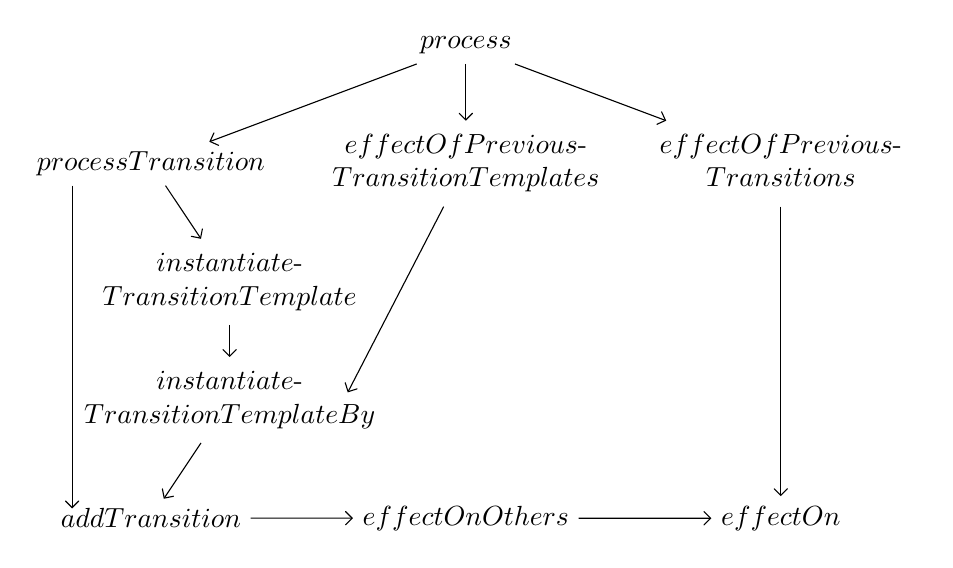
\begin{tikzpicture}[>=angle 90,yscale = 1.5]
\draw (0,0) node (process) {$process$};
\draw (process) ++ (-4,-1) node (processTransition) {$processTransition$};
%
\path[draw,->] (process) -- (processTransition);
\draw (process) ++ (0,-1) node (effectPrevTT)
   {$\begin{array}{c} effectOfPrevious\mbox{-} \\ 
       TransitionTemplates\end{array}$}; 
\path[draw,->] (process) -- (effectPrevTT);
\draw (process) ++ (4,-1) node (effectPrevTrans) 
  {$\begin{array}{c} effectOfPrevious\mbox{-} \\ Transitions\end{array}$}; 
\path[draw,->] (process) -- (effectPrevTrans);
%
\draw (processTransition) ++ (1,-1) node (instantiateTT) 
  {$\begin{array}{c} instantiate\mbox{-}\\ TransitionTemplate \end{array}$};
\path[draw,->] (processTransition) -- (instantiateTT);
%
\draw (instantiateTT) ++ (0,-1) node (instantiateTTBy)
  {$\begin{array}{c} instantiate\mbox{-}\\ TransitionTemplateBy \end{array}$};
\path[draw,->] (instantiateTT) -- (instantiateTTBy);
\path[draw,<-] (instantiateTTBy.north)++(1.5,-0.3) -- (effectPrevTT);
%
\draw (instantiateTTBy) ++ (-1,-1) node (addTransition) {$addTransition$};
\path[draw,->] (instantiateTTBy) -- (addTransition);
\draw (addTransition)++(-1,0) node (addTransitionL) {};
\path[draw,->] (processTransition.south)++(-1,0) -- (addTransitionL);
%
\draw (addTransition) ++ (4,0) node (effectOnOthers) {$effectOnOthers$};
\path[draw,->] (addTransition) -- (effectOnOthers);
%
\draw (effectOnOthers) ++ (4,0) node (effectOn) {$effectOn$}; 
\path[draw,->] (effectOnOthers) -- (effectOn);
\path[draw,->] (effectPrevTrans) -- (effectOn);
\end{tikzpicture}
\end{center}
\caption{Relationship of functions}
\label{fig:impl}
\end{figure}

The function $process(v)$ acts on a single view~$v$ found on the previous ply.
It calculates all the transitions from~$v$, together with the identities of
other components relevant to the view (if any).  It then calls
$processTransition$ on each such transition.  It also calls
$effectOfPreviousTransitions$ and $effect\-Of\-Previous\-TransitionTemplates$
on the view.

The function $processTransition(pre, e, post, ids)$ corresponds to processing
either (1)~the transition $pre \trans{e} post$, if $ids$ is empty, or
(2)~transition template $(pre, post, id, e, true)$ if $ids = \set{id}$,
i.e.~transitions with an extra component with identity~$id$ that synchronises
on~$e$.  It calculates whether the principal component gains a reference to a
component other than those in~$pre$ and~$id$.  If not and $ids$ is empty, the
transition is complete: $addTransition$ is called on it.  Otherwise, it is
added to $newTransitionTemplates$, and
$instantiate\-TransitionTemplate$ is called.

$addTransition(pre,e,post)$ adds a transition $pre \trans{e} post$ to
$new\-Transitions$, and calls $effectOnOthers$.

$effectOnOthers(pre,e,post)$ considers the effect of a new transition $pre
\trans{e} post$ on views found on previous plys.  For each such view that
matches $pre$'s fixed processes, it calls $effectOn$.

$effectOn(pre, e, post, v)$ considers the effect of a transition $pre
\trans{e} post$ on another view~$v$.  It forms all ways of combining $pre$ and
$v$, calculates the corresponding post-view for $v.\princ$, and adds it to
$nextNewViews$.

$instantiateTransitionTemplate(pre, post, id, e, inc)$ considers how to
instantiate the transition template $(pre, post,\linebreak[1] id,\linebreak[1]
e, inc)$.  For each view in $sysAbsViews$ that matches $pre$'s fixed
processes, it calls $instantiate\-Transition\-TemplateBy$.

$instantiateTransitionTemplateBy(pre, post, id, e, inc, v)$ considers how
to instantiate the transition template $(pre, post,\linebreak[1]
id,\linebreak[1] e, inc)$, so that a component of $v$ forms the extra
component with identity~$id$.  For each resulting transition, it calls
$add\-Transition$.

$effectOfPreviousTransitions(v)$ considers the effect of all previous
transitions on a view~$v$ found on the previous ply.  For each
transition in $transitions$ whose initial servers matches $v$'s servers, it
calls $effectOn$.

$effectOfPreviousTransitionTemplates(v)$ considers using a view~$v$ found on
the previous ply to instantiate the missing component in a transition
template.  For each transition template in $transitionTemplates$ whose initial
servers matches $v$'s servers, it calls $instantiateTransitionTemplateBy$.

We briefly discuss the combination of views and either transitions or
transition templates: it is important that we consider each such combination,
just once, regardless of the plys each are found or created on.  Consider a
view~$v$ found on ply~$n$, and expanded on ply~$n+1$.
%
\begin{itemize}
\item On ply~$n+1$, $v$ will be considered (in $effectOfPreviousTransitions$)
  in combination with each transition created up to ply~$n$.

\item For each transition created on ply~$n+1$ or later, its effect on~$v$
  will be considered (in $effectOnOthers$) on the ply in which the transition
  is created. 
 %% A transition from~$v$ will be considered in ply~$n+1$, and its effect
 %%  considered (in $effectOnOthers$) on all views~$v'$ found up to ply~$n$.
\end{itemize}
%
Thus the combination of a view and a transition will be treated: (1)~by the
first bullet if the transition is created on a ply no later than the view is
found; and (2)~by the second bullet if the transition is created on a ply
later than the view is found.  

Likewise
%
\begin{itemize}
\item On ply $n+1$, $v$ will be considered (in
  $effect\-Of\-Previous\-Transition\-Templates$) to create the missing
  component in each transition template created up to ply~$n$.

\item For each transition template created on ply~$n+1$ or later, its
  combination with~$v$ will be considered (in
  $instantiate\-Transition\-Template$) on the ply in which the transition
  template is created.
%% \item A transition template from~$v$ will be created in ply~$n+1$, and all
%%   ways of creating the missing component from views found up to ply~$n$ will
%%   be considered (in $instantiateTransitionTemplate$).
\end{itemize}
%
Thus the combination of a view and a transition template will be treated:
(1)~by the first bullet if the transition template is created on a ply no
later than the view is found; and (2)~by the second bullet if the transition
template is created on a ply later than the view is found.

%%%%%%%%%%%%%%%%%%%%%%%%%%%%%%%%%%%%%%%%%%%%%%%%%%%%%%%

\subsection{instantiateTransitiontemplateBy}

$instantiateTransitionTemplateBy(pre, post, id, e, inc, v)$ considers how
to instantiate the transition template $(pre, post,\linebreak[1]
id,\linebreak[1] e, inc)$, so that a component of $v$ forms the extra
component with identity~$id$.  For each resulting transition, it calls
$add\-Transition$.


The function $consistentStates(pre, id, e, inc, v)$ considers how to rename
$v$ to potentially produce the extra component of the transition template
$(pre, post,\linebreak[1] id,\linebreak[1] e, inc)$.  More precisely, it finds
all ways of renaming~$v$ to obtain a view~$v'$ so that (1) a component of~$v'$
has identity~$id$, (2)~$v'$ and~$pre$ agree on common components, and (3)~if
$inc$ then $v'$ can perform~$e$.  For each, it returns the renamed component
with identity id, and the next states. 

For each such extra component~$st$,\, $isExtendable(pre, st)$ tests whether
$st$ is consistent with $pre$, in the sense that for each component $c$ of
$pre \union st$, the current set of views contains a view with $c$ as
principal component and agreeing on common processes (modulo renaming).

$compatibleWith(servers, components, st)$ tests whether there is an existing
view with $st$ as principal component that agrees with $servers$ and
$components$ on common processes. 

$containsReferencingView(pre, st, j)$ assumes that $pre.components(j)$ has a
reference to $st$.  If tests whether there is a view with $pre.components(j)$
as principal component, containing $st$, and otherwise compatible with~$pre$
(modulo renaming).

*** If the views that ensure consistency are found later, do we get all
instantiations?  I think so.  The last relevant view will include the state we
want. 


%%%%%%%%%%%%%%%%%%%%%%%%%%%%%%%%%%%%%%%%%%%%%%%%%%%%%%%


\end{document}
